\documentclass{report}
\usepackage[utf8]{inputenc}

\usepackage{cite}
\usepackage{booktabs}
\usepackage{amsmath}
\usepackage{amssymb}
\usepackage[dvipsnames]{xcolor}
\usepackage[pdftex]{graphicx}
\usepackage{subcaption}
\usepackage{hyperref}
\hypersetup{
  colorlinks,
  linktoc=all
  citecolor=black,
  filecolor=black,
  linkcolor=black,
  urlcolor=black
}

% Paragraph settings
\setlength{\parindent}{1em}
\setlength{\parskip}{1.0em}


% Linear algebra
\renewcommand{\Vec}[1]{{\mathbf{#1}}}
\newcommand{\Mat}[1]{{\mathbf{#1}}}
\newcommand{\real}{{\rm I\!R}}
\newcommand{\ones}{{\Vec{1}}}
\newcommand{\Ones}[2]{{\Vec{1}_{#1\times#2}}}
\newcommand{\zeros}{{\Vec{0}}}
\newcommand{\Zeros}[2]{{\Vec{0}_{#1\times#2}}}
\newcommand{\Norm}[1]{{\|#1\|}}
\newcommand{\LargeNorm}[1]{{\left\lVert#1\right\rVert}}
\newcommand{\I}{{\Mat{I}}}
\newcommand{\quat}{{\Vec{q}}}
\newcommand{\jac}{{\Mat{J}}}
\newcommand{\Skew}[1]{{\lfloor #1 \enspace \times \rfloor}}
\newcommand{\Argmin}[1]{\underset{#1}{{\text{argmin }}}}
\newcommand{\transpose}{T}
\newcommand{\Transpose}[1]{{{#1^{\transpose}}}}
\newcommand{\Inv}[1]{{{#1^{-1}}}}
\newcommand{\LargeNorm}[1]{\left\lVert#1\right\rVert}
\newcommand{\Trace}[1]{\text{tr}(#1)}
\newcommand{\Rank}[1]{\text{rank}(#1)}
\newcommand{\Bigslant}[2]{{\raisebox{.2em}{$#1$}\left/\raisebox{-.2em}{$#2$}\right.}}


% Frames
\newcommand{\tf}{\mathbf{T}}
\renewcommand{\frame}{\mathcal{F}}
\newcommand{\body}{{\text{B}}}
\newcommand{\cam}{{\text{C}}}
\newcommand{\robot}{{\text{R}}}
\newcommand{\sensor}{{\text{S}}}
\newcommand{\world}{{\text{W}}}
\newcommand{\worldb}{{\text{G}}}
\newcommand{\fiducial}{{\text{F}}}
% -- Kinematic Notation --
% ---- Paul Furgale Kinematic Notation ----
\newcommand{\KineNotation}[3]{{{{}_{#2}} {#1}_{#2#3}}}
\newcommand{\KineNotationProper}[4]{{{{}_{#2}} {#1}_{#3#4}}}
\newcommand{\KineNotationPart}[3]{{{{}_{#2}} {#1}_{#3}}}
\newcommand{\KineNotationBare}[2]{{{{}_{#2}} {#1}}}
\newcommand{\KineNotationTransform}[3]{{{#1}_{#2#3}}}
% -- Translation --
\newcommand{\trans}{{\Vec{r}}}
\newcommand{\Trans}[2]{{\KineNotation{\trans}{#1}{#2}}}
% -- Position --
\newcommand{\pos}{{\Vec{r}}}
\newcommand{\Pos}[2]{{\KineNotation{\pos}{#1}{#2}}}
\newcommand{\DotPos}[2]{{\KineNotation{\dot{\pos}}{#1}{#2}}}
% -- Velocity --
\newcommand{\vel}{{\Vec{v}}}
\newcommand{\Vel}[2]{{\KineNotation{\vel}{#1}{#2}}}
\newcommand{\DotVel}[2]{{\KineNotation{\dot{\vel}}{#1}{#2}}}
% -- Angular Velocity --
\newcommand{\angvel}{{\boldsymbol{\omega}}}
\newcommand{\AngVel}[2]{{\KineNotation{\angvel}{#1}{#2}}}
\newcommand{\PAngVel}[3]{{\KineNotationProper{\angvel}{#1}{#2}{#3}}}
\newcommand{\PAngVelMeas}[3]{{\KineNotationProper{\tilde{\angvel}}{#1}{#2}{#3}}}
% -- Acceleration --
\newcommand{\acc}{{\Vec{a}}}
\newcommand{\Acc}[2]{{\KineNotation{\acc}{#1}{#2}}}
\newcommand{\PAcc}[3]{{\KineNotationProper{\acc}{#1}{#2}{#3}}}
\newcommand{\PAccMeas}[3]{{\KineNotationProper{\tilde{\acc}}{#1}{#2}{#3}}}
% -- Rotation --
\newcommand{\dtheta}{{\delta{\boldsymbol{\theta}}}}
\newcommand{\rot}{{\Mat{C}}}
\newcommand{\Rot}[2]{{\KineNotationTransform{\rot}{#1}{#2}}}
\newcommand{\Quat}[2]{{\KineNotationTransform{\quat}{#1}{#2}}}
\newcommand{\DotQuat}[2]{{\KineNotationTransform{\dot\quat}{#1}{#2}}}
% -- Transforms --
\newcommand{\tf}{{\Mat{T}}}
\newcommand{\Tf}[2]{{\KineNotationTransform{\tf}{#1}{#2}}}
% -- Point --
\newcommand{\point}{\Vec{p}}
\newcommand{\Pt}[1]{{\KineNotationPart{\point}{#1}{}}}
\newcommand{\Point}[2]{{\KineNotationBare{\point}{#1}}}

% Variables
% -- Probability
\newcommand{\RV}[1]{\mathbf{#1}}
% -- Computer vision
\newcommand{\dalpha}{{\delta\boldsymbol{\alpha}}}
\newcommand{\error}{{\Vec{e}}}
\newcommand{\camQuat}{{\Quat{\world}{\cam}}}
\newcommand{\camRot}{{\Rot{\world}{\cam}}}
\newcommand{\camPos}{{\Pos{\world}{\cam}}}
\newcommand{\projFunc}{{\Vec{h}}}
\newcommand{\errFunc}{{\Vec{e}}}
\newcommand{\measurement}{{\Vec{z}}}
\newcommand{\estimate}{{\tilde{\Vec{z}}}}
% -- IMU
\newcommand{\imuAccel}{{\PAcc{\sensor}{\world}{\sensor}}}
\newcommand{\imuGyro}{{\PAngVel{\sensor}{\world}{\sensor}}}
\newcommand{\imuAccelMeas}{{\PAccMeas{\sensor}{\world}{\sensor}}}
\newcommand{\imuGyroMeas}{{\PAngVelMeas{\sensor}{\world}{\sensor}}}
\newcommand{\noise}{{\mathbf{w}}}
\newcommand{\noiseGyro}{{\noise_{g}}}
\newcommand{\noiseAccel}{{\noise_{a}}}
\newcommand{\bias}{{\mathbf{b}}}
\newcommand{\biasGyro}{{\bias_{g}}}
\newcommand{\biasAccel}{{\bias_{a}}}
\newcommand{\gravity}{{\mathbf{g}_{\world}}}


\begin{document}

% TABLE OF CONTENTS
\tableofcontents

% CHAPTERS
\chapter{Notations}

A large part of robotics is about developing machines that perceives and
interact with the environment. For that robots use sensors to collect and
process data, and knowing what the data describes is of utmost importance.
Imagine obtaining the position of the robot but not knowing what that position
is with respect to. Missing data descriptions such as what a position vector is
expressing, what is it with respect to and more causes many hours of painful
trail and error to extract that information.

In the following section the notation used throughout this document will be
described, and it follows closely of that of Paul Furgale's~\cite{Furgale2014}.
The aim is to mitigate the ambiguity that arises when describing robot poses,
sensor data and more.

A vector expressed in the world frame, $\frame_{\world}$, is written as
$\KineNotationBare{\pos}{\world}$. Or more precisely if the vector describes
the position of the camera frame, $\frame_{\cam}$, expressed in
$\frame_{\world}$, the vector can be written as $\Pos{\world}{\cam}}$ with
$\world$ and $\cam$ as start and end points. The left hand subscripts indicates
the coordinate system the vector is expressed in, while the right-hand
subscripts indicate the start and end points. For brevity if the vector has
the same start point as the frame to which it is expressed in, the same vector
can be written as $\KineNotationPart{\pos}{\world}{\cam}$. Similarly a
transformation of a point from $\frame_{\cam}$ to $\frame_{\world}$ can be
represented by a homogeneous transform matrix, $\Tf{\world}{\cam}$, where its
rotation matrix component is written as $\Rot{\world}{\cam}$ and the
translation component written as $\Trans{\world}{\cam}$. A rotation matrix that
is parametrized by quaternion $\quat_{\world\cam}$ is written as
$\rot\{\quat_{\world\cam}\}$.



\begin{align*}
  &\text{Position:} \enspace & \Pos{\world}{\body} \\
  &\text{Velocity:} \enspace & \Vel{\world}{\body} \\
  &\text{Acceleration:} \enspace & \Acc{\world}{\body} \\
  &\text{Angular velocity:} \enspace & \AngVel{\world}{\body} \\
  &\text{Rotation:} \enspace & \Rot{\world}{\body} \\
  &\text{Transform:} \enspace & \Tf{\world}{\body} \\
  &\text{Point:} \enspace & \Pt{\world}
\end{align*}

\chapter{Statistics}



% MEAN
\section{Mean}

\begin{equation}
  \mu = \dfrac{1}{N} \sum_{i=1}^{N} x_{i}
\end{equation}



% VARIANCE
\section{Variance}

Variance is a measure of spread, it is the average squared distance between
measurements and the mean.

The Population variance is defined as,
%
\begin{equation}
  \sigma^{2} = \dfrac{\sum_{i=1}^{N} (x_i - \mu)^{2}}{N}.
\end{equation}

The Sample variance is defined as,
%
\begin{equation}
  \sigma^{2} = \dfrac{\sum_{i=1}^{n} (x_i - \mu)^{2}}{n - 1}.
\end{equation}

Where $N$ is the population size and $n$ is the sample size.

In plain english, the population variance, standard deviation, etc, is when the
whole population data is available. Sample variance, standard deviation, etc,
on the other hand implies the availble data is only a subset of the population.

The problem with sample data is that estimates without applying the $n - 1$
correction will often underestimate the true value. This is particularly true
if $n$ is small. By using $n - 1$ instead of $n$ as the divsor corrects the
estimate by making the result slightly larger.

The degrees of freedom is another perspective of why $n - 1$ should be use when
estimating from sample data. In statistics the degrees of freedom describe the
number variables that could affect the response or output of a model. (need
more explaining)



% STANDARD DEVIATION
\section{Standard Deviation}

The standard deviation $\sigma$ is defined as the square root of the variance
$\sigma^{2}$. It is also a measure of spread in the data. However standard
deviation is often more intuitive, because instead of the spread in terms of
distance from the \textit{mean squared}, the standard deviation is simply the
distance from the mean (not \textit{mean squared}).

\begin{equation}
  \sigma = \sqrt{\sigma^2}
\end{equation}



% STANDARD ERROR
\section{Standard Error}

Standard error of the regression, or standard error of the estimate is the
average distance between observed values and the fitted model. This metric
conveys objectively how wrong the regression model is on average using the
units of the response variable. A small standard error indicates observations
are closer to the fitted model. Conceptually it is similar to the standard
deviation, the difference is standard deviation measures te average distance of
the observed alues from the mean.

The standard error (S) is defined as:
%
\begin{equation}
  S = \sqrt{\dfrac{\sum_{i=1}^{n} (\hat{y}_{i} - y_{i})^{2}}{df}}
\end{equation}



% Pearson's Chi-Squared Test
\section{Pearson's Chi-Squared Test}

Pearson's chi-squared test $\chi^2$ is a statistical test applied to sets of
\textit{categorial data} to quantify the likelihood that the observed
difference between measured and predicted arose by chance. The test is used to
assess three types of comparisons:
%
\begin{itemize}
  \item{\textbf{Goodness of fit}: checks whether the observed frequency
    distribution matches the theoretical distribution.}
  \item{\textbf{Homogeneity}: compares the distribution of counts for two or
    more groups using the same categorical variable.}
  \item{\textbf{Independence}: checks whether the unparied observations on two
    variables, expressed in a contingency table, are independent of each
    other.}
\end{itemize}


\subsection{Goodness of Fit}

\begin{equation}
  \chi^2 = \sum^{n}_{i=1} \dfrac{(O_i - E_i)^2}{E_i} \\
    = N \sum^{n}_{i=1} \dfrac{(O_i / N - p_i)^2}{p_i}
\end{equation}
%
where $\chi^2$ is Pearson's cumulative test statistic, $O_i$ is the number of
observations of type $i$, $N$ is the total number of observations, $E_i = N
p_i$ is the expected (theoretical) count of type $i$, and $n$ is the number of
cells in the table.

Once the chi-squared test statistic is calculated, the $p$-value is obtained by
comparing the value of the statistic to a chi-squared distribution. The number
of degrees of freedom is equal to the number of cells $n$, minus the reduction
in degrees of freedom, $p$.

\subsubsection{Example: Fairness of dice}

A 6-sided die is thrown 60 times. The number of times it lands with 1, 2, 3, 4,
5 and 6 face up is 5, 8, 9, 8, 20 and 20, respectively. Is the die biased,
according to the Pearson's chi-squared test at a significance level of 95\%,
and, or 99\%?

In this example $n = 6$ as there are 6 possible outcomes, 1 to 6. The null
hypothesis is that the die is unbaised, hence each dice number is expected to
occur the same number of times, in this case, $60 / n = 10$. The outcomes can
be tabulated as follows:
%
\begin{table}[h]
  \center
  \begin{tabular}{cccccc}
    \toprule
    $i$
    & $O_i$
    & $E_i$
    & $O_i - E_i$
    & $(O_i - E_i)^2$
    & $\dfrac{(O_i - E_i)^2}{E_i}$ \\
    \hline
    1 & 5 & 10 & -5 & 25 & 2.5 \\
    2 & 8 & 10 & -2 & 4 & 0.4 \\
    3 & 9 & 10 & -1 & 1 & 0.1 \\
    4 & 8 & 10 & -2 & 4 & 0.4 \\
    5 & 10 & 10 & 0 & 0 &  0 \\
    6 & 20 & 10 & 10 & 100 & 10 \\
    \hline
    & & & & Sum: & 13.4 \\
    \bottomrule
  \end{tabular}
\end{table}

The number of degrees of freedom is $n - 1 = 5$. The Upper tail critical values
of chi-square distribution gives a critical value of 11.070 at 95\%
significance level:
%
\begin{table}[h]
  \center
  \begin{tabular}{p{1.6cm} | ccccc}
    Degrees of Freedom
    & \multicolumn{5}{c}{Probability less than the critical value} \\
    & \textbf{0.90}
    & \textbf{0.95}
    & \textbf{0.975}
    & \textbf{0.99}
    & \textbf{0.999} \\
    \hline
    5 & 9.236 & 11.070 & 12.833 & 15.086 & 20.515
  \end{tabular}
\end{table}
%
As the chi-squared statistic of 13.4 exceeds this critical value, the null
hypothesis is rejected and conclude that the die is biased at 95\% significance
level. At 99\% significance level, the critical value is 15.086. As the
chi-squared statistic does not exceed it, the null hypothesis
is not rejected and thus conclude that there is insufficient evidence to show
that the die is biased at 99\% significance level.


\subsection{Problems with Pearson's Chi-Squared Test~\cite{Andrae2010}}

\begin{itemize}
  \item{The degrees of freedom can only be estimated for \textit{linear
    models}. It is non-trivial or near impossible to estimate the degrees of
    freedom for a \textit{non-linear model}.}
  \item{The value of chi-squared itself is subject to noise in the data, as
    such the value is uncertain.}
\end{itemize}

Knowing the degrees of freedom of the model in question is required for
chi-squared test. For $N$ data points and $P$ parameters, a naive guess is that
the number of degrees of freedom is $N - P$. This, however, as will be
demonstrated is not always the case.

The chi-squared test statistic, $\chi^2$, for continuous data is defined as,
%
\begin{equation}
  \chi^2 = \sum^{N}_{n = 1}
    \left( \dfrac{(y_n - f(x_n, \theta))}{\sigma_n} \right)^2
\end{equation}
%
which is equivalent to maximizing the liklihood function. For a linear model,
the chi-squared statistic, $\chi^2$ can be written in matrix form as,
%
\begin{equation}
  \chi^2 =
    (\Vec{y} - \Mat{X} \boldsymbol{\theta})^{\transpose}
    \Mat{\Sigma}^{-1}
    (\Vec{y} - \Mat{X} \boldsymbol{\theta}) .
\end{equation}
%
Rearranging in terms of the model parameters, $\boldsymbol{\theta}$, gives,
\begin{equation}
  \boldsymbol{\theta} =
    (\Mat{X}^{\transpose} \Mat{\Sigma}^{-1} \Mat{X})^{-1}
    \Mat{X}^{\transpose} \Mat{\Sigma}^{-1} \Vec{y} .
\end{equation}
%
Finally, the prediction, $\hat{\Vec{y}}$, of the measurements, $\Vec{y}$, can
be obtained by multiplying the design matrix, $\Mat{X}$, with the model
parameters, $\boldsymbol{\theta}$, and further simplified to give us,
%
\begin{align}
  \hat{\Vec{y}}
    &= \Mat{X} \boldsymbol{\theta} \\
    &= \Mat{X} (\Transpose{\Mat{X}} \Mat{\Sigma}^{-1} \Mat{X})^{-1}
       \Transpose{\Mat{X}} \Mat{\Sigma}^{-1} \Vec{y} \\
    &= \Mat{H} \Vec{y}
\end{align}
%
where $\Mat{H}$ is an $N \times N$ matrix, sometimes called the ``hat matrix''
because it translates the measurement data, $\Vec{y}$, into a model prediction,
$\hat{\Vec{y}}$. The number of \textit{effecitve} model parameters,
$P_{\text{eff}}$, is then given by the trace of $\Mat{H}$,
%
\begin{equation}
  P_{\text{eff}} = \Trace{\Mat{H}} = \sum^{N}_{n = 1} H_{nn} = \Rank{\Mat{X}} .
\end{equation}
%
which also equals the rank of the design matrix $\Mat{X}$. And so,
$P_{\text{eff}} \leq P$, where the equality holds if and only if the design
matrix $\Mat{X}$ has full rank. Consequently, for linear models the number of
degrees of freedom is,
%
\begin{equation}
  K = N - P_{\text{eff}} \geq N - P
\end{equation}
%
For nonlinear models, the degrees of freedom is not as straight forward.


\subsubsection{Example 1}

Let us consider a nonlinear model with three free parameters, $A$, $B$, and $C$,
%
\begin{equation}
  f(x) = A \cos(Bx + C) .
\end{equation}
%
If we are given a set of $N$ measurement $(x_n, y_n, \sigma_n)$ such that no
two data points have identical $x_n$, then the model $f(x)$ is capable of
fitting any such data set perfectly. The way this works is by increasing the
``frequency'' $B$ such that $f(x)$ can change on arbitrarily short scales. As $f(x)$
provides a perfect fit in this case, $\chi^2$ is equal to zero for all possible
noise realizations of the data. Evidently, this three-parameter model has
infinite flexibility (if there are no priors) and $K = N - P$ is a poor estimate
of the number of degrees of freedom, which actually is $K = 0$.


\subsubsection{Example 2}

To build upon the first example, three additional model parameters, $D$, $E$
and $F$ are added,
%
\begin{equation}
  f(x) = A \cos(Bx + C) + D \cos(Ex + F) .
\end{equation}
%
If the fit parameter $D$ becomes small such that $|D| \leq |A|$, the second
component cannot influence the fit anymore and the two model parameters $E$ and
$F$ are ``lost''. In simple words: This model may change its flexibility during
the fitting procedure.

Hence, for nonlinear models, K may not even be constant. Of course, these two
examples do not verify the claim that always $K \neq N - P$ for nonlinear
models.  However, acting as counter-examples, they clearly falsify the claim
that $K = N - P$ is always true for nonlinear models.



\chapter{Linear Algebra}


% TRACE
\section{Trace}

\begin{equation}
  \text{tr}(\Mat{A}) = \sum_{i} \Mat{A}_{ii}
\end{equation}



% RANK
\section{Rank}

The rank $\rho(\Mat{A})$ of a matrix $\Mat{A}$ of $n$ rows and $m$ columns is
defined as \textbf{the number of independent rows or columns}.

\begin{itemize}
  \item{Full rank (non-singular): $\rho(\Mat{A}) = \min(n, m)$}
  \item{Not full rank (singular): $\rho(\Mat{A}) < \min(n, m)$}
\end{itemize}



% CONDITION NUMBER FOR INVERSION
\section{Condition Number}

There are different condition numbers in the following the condition number for
the problem $\Mat{A} \Vec{x} = \Vec{b}$ and matrix inversion are discussed. In
general, the condition number, $\kappa(\cdot)$, for a matrix, $\Mat{A}$, or
computational task such as $\Mat{A} \Vec{x} = \Vec{b}$ measures how sensitive
the output is to perturbations in the input data and to round off errors. If
the condition number is large, even a small error in $\Vec{x}$ would cause a
large error in $\Vec{x}$. On the other hand, if the condition number is small
then the error in $\Vec{x}$ will not be much bigger than the error in
$\Vec{b}$.
%
\begin{align}
  \kappa(\Mat{A}) &\approx 1 \quad \text{well-Conditioned} \\
  \kappa(\Mat{A}) &> 1 \quad \text{ill-Conditioned}
\end{align}

The condition number is defined more precisely to be the maximum ratio of the
relative error in $\Vec{x}$ to the relative error in $\Vec{b}$.

Let $\Vec{e}$ be the error in $\Vec{b}$. Assuming that $\Mat{A}$ is a
nonsingular matrix, the error in the solution $\Mat{A}^{-1} \Vec{b}$ is
$\Mat{A}^{-1} \Vec{e}$. The ratio of the relative error in the solution to the
relative error in $\Vec{b}$ is
%
\begin{equation}
  \Bigslant{
    \dfrac{\Norm{\Mat{A}^{-1} \Vec{e}}}{\Norm{\Mat{A}^{-1} \Vec{b}}}
  }{
    \dfrac{\Norm{\Vec{e}}}{\Norm{\Vec{b}}}
  }
\end{equation}
%
which can be rewritten as,
%
\begin{equation}
  \left(
    \dfrac{\Norm{\Mat{A}^{-1} \Vec{e}}}{\Norm{\Vec{e}}}
  \right)
  \cdot
  \left(
    \dfrac{\Norm{\Vec{b}}}{\Norm{\Mat{A}^{-1} \Vec{b}}}
  \right)
\end{equation}
%
The maximum value (for nonzero $\Vec{b}$ and $\Vec{e}$) is then seen to be the
product of the two operator norms as follows:
%
\begin{align}
  % -- LINE 1
  &\max_{\Vec{e}, \Vec{b} \neq 0}
  \left\{
    \left(
      \dfrac{\Norm{\Mat{A}^{-1} \Vec{e}}}{\Norm{\Vec{e}}}
      \cdot
      \dfrac{\Norm{\Vec{b}}}{\Norm{\Mat{A}^{-1} \Vec{b}}}
    \right)
  \right\} \\
  % -- LINE 2
  &= \max_{\Vec{e}, \Vec{b} \neq 0}
  \left\{
    \left(
      \dfrac{\Norm{\Mat{A}^{-1} \Vec{e}}}{\Norm{\Vec{e}}}
    \right)
  \right\}
  \cdot
  \max_{\Vec{e}, \Vec{b} \neq 0}
  \left\{
    \left(
      \dfrac{\Norm{\Vec{b}}}{\Norm{\Mat{A}^{-1} \Vec{b}}}
    \right)
  \right\} \\
  % -- LINE 3
  &= \max_{\Vec{e}, \Vec{b} \neq 0}
  \left\{
    \left(
      \dfrac{\Norm{\Mat{A}^{-1} \Vec{e}}}{\Norm{\Vec{e}}}
    \right)
  \right\}
  \cdot
  \max_{\Vec{e}, \Vec{b} \neq 0}
  \left\{
    \left(
      \dfrac{\Norm{\Mat{A} \Vec{x}}}{\Norm{\Vec{x}}}
    \right)
  \right\} \\
  % -- LINE 4
  &= \Norm{\Mat{A}^{-1}} \cdot \Norm{\Mat{A}}
\end{align}
%
The same definition is used for any matrix norm, i.e. one that satisfies
%
\begin{equation}
  \kappa(\Mat{A}) = \Norm{\Mat{A}^{-1}} \cdot \Norm{\Mat{A}}
    \geq \Norm{\Mat{A}^{-1} \cdot \Mat{A}} = 1 .
\end{equation}
%
When the condition number is exactly one (which can only happen if $\Mat{A}$ is
a scalar multiple of a linear isometry), then a solution algorithm can find (in
principle, meaning if the algorithm introduces no errors of its own) an
approximation of the solution whose precision is no worse than that of the
data.

However, it does not mean that the algorithm will converge rapidly to this
solution, just that it won't diverge arbitrarily because of inaccuracy on the
source data (backward error), provided that the forward error introduced by the
algorithm does not diverge as well because of accumulating intermediate
rounding errors.

The condition number may also be infinite, but this implies that the problem is
ill-posed (does not possess a unique, well-defined solution for each choice of
data -- that is, the matrix is not invertible), and no algorithm can be
expected to reliably find a solution.

The definition of the condition number depends on the choice of norm, as can be
illustrated by two examples.

\chapter{Probability Theory}

\section{Bayes Theorem}

\begin{equation}
  p(\RV{x}, \RV{y}) = p(\RV{x}|\RV{y}) p(\RV{y}) = p(\RV{x}|\RV{y}) p(\RV{y})
\end{equation}

\begin{equation}
  \underbrace{p(\RV{x}|\RV{y})}_{\text{Posterior}} =
    \dfrac{
      \overbrace{p(\RV{x}|\RV{y})}^{\text{Likelihood}}
      \enspace
      \overbrace{p(\RV{y})}^{\text{Prior}}
    }{
      \underbrace{p(\RV{y})}_{\text{Evidence}}
    }
\end{equation}

\chapter{Computer Vision}

\section{Fundamentals}

\subsection{Point on Line}

\begin{equation}
  \Transpose{\Vec{x}} \Vec{l} = 0
\end{equation}


\subsection{Intersection of Lines}

\begin{equation}
  \Vec{l} (\Vec{l} \times \Vec{l}')
  \Vec{l}' (\Vec{l} \times \Vec{l}')
  = 0 \\
  \Transpose{\Vec{l}} \Vec{x}
  = \Transpose{\Vec{l}}' \Vec{x}
  = 0
\end{equation}

\begin{equation}
  x = \Vec{l} \times \Vec{l}'
\end{equation}


\subsection{Plane}

\begin{itemize}
  \item{A plane can be defined by the join between three points, or the join
        between a line and a point in general}
  \item{Two planes intersecting a unique line}
  \item{Three planes intersecting a unique point}
\end{itemize}

\subsubsection{Three Points Define a Plane}

Suppose you have three points $\Vec{X}_{1}$, $\Vec{X}_{2}$, $\Vec{X}_{3}$, and
are incident with a plane, $\pi$ then each point satisfies
%
\begin{equation}
  \Transpose{\pi} \Vec{X}_{i} = 0.
\end{equation}
%
By stacking each point as a matrix
%
\begin{align}
  \begin{bmatrix}
    \Transpose{\Vec{X}_{1}} \\
    \Transpose{\Vec{X}_{2}} \\
    \Transpose{\Vec{X}_{3}}
  \end{bmatrix} \pi = 0
\end{align}
%
Since three points in general rare linearly independent, it follows that the
$3x4$ matrix compsed of the points $\Vec{X}_{i}$ as rows has rank 3.


\subsection{Fundamental Matrix}

\subsection{Essential Matrix}



% PINHOLE CAMERA MODEL
\section{Pinhole Camera Model}

The pinhole camera model describes how 3D scene points are projected onto the
2D image plane of an ideal pinhole camera. The model makes the assumption that
light rays emitted from an object in the scene pass through the pinhole of the
camera, and projected onto the image plane. A 3D point $\mathbf{X}_{C} = (X, Y,
Z)$ expressed in the camera frame, $\frame_{C}$, projected on to a camera's 2D
image plane in homogeneous coordinates $\mathbf{x}_{C} = (u, v, 1)$ can be
written as
%
\begin{equation}
  u = \dfrac{X f_{x}}{Z} \quad v = \dfrac{Y f_{y}}{Z}
\end{equation}
%
where $f_{x}$ and $f_{y}$ denote the focal length in the x and y-axis. Or, in
matrix form
%
\begin{align}
	\mathbf{x}_{C} &= \mathbf{K} \mathbf{X}_{C} \\
	\begin{bmatrix}
		u \\ v \\ 1
	\end{bmatrix} &=
	\begin{bmatrix}
		f_{x} & 0 & c_{x} \\
		0 & f_{x} & c_{y} \\
		0 & 0 & 1
	\end{bmatrix}
	\begin{bmatrix}
		X / Z \\ Y / Z \\ 1
	\end{bmatrix}
\end{align}
%
where $\mathbf{K}$ represents the intrinsic matrix, $c_{x}$ and $c_{y}$
represents the principal point offset in the $x$ and $y$ direction.

In practice, the pinhole camera model only serves as an approximation to modern
cameras. The assumptions made in the model are often violated with factors such
as large camera apertures (pinhole size), distortion effects in camera lenses,
and other factors. That is why the pinhole camera model is often used in
combination with a distortion model in the hope of minimizing projection errors
from 3D to 2D.



% Radial Tangential Distortion
\section{Radial Tangential Distortion}

Lens distortion generally exist in all camera lenses, therefore it is vital we
model the distortions observed. The most common distortion model is the
radial-tangential (or simply as radtan) distortion model. The two main
distortion components, as the name suggests, are the radial and tangential
distortion.

The radial distortion occurs due to the shape of the lens. Light passing
through the center undergoes no refraction. Light passing through the edges of
the lens, on the other hand, undergoes through severe bending causing the
radial distortion. The effects of a positive and negative radial distortion can
be seen in Fig~\ref{fig:radial_distortion}.

The tangential distortion is due to camera sensor misalignment during the
manufacturing process. It occurs when the camera sensor is not in parallel with
the lens. The cause of a tangential distortion can be seen in
Fig~\ref{fig:tangential_distortion}.

The combined radial-tangential distortion is modelled using a polynomial
approximation with parameters $k_{1}, k_{2}$ and $p_{1}, p_{2}$ respectively.
To apply the distortion the observed 3D point $(X, Y, Z)$ is first projected,
distorted, and finally scaled and offset in the image plane $(u, v)$. The
radial-tangential distortion model in combination with the pinhole camera model
is given in Eq.~\eqref{eq:radtan_pinhole} as
%
\begin{align}
  \begin{split}
    x &= X / Z \\
    y &= Y / Z \\
    r^2 &= x^2 + y^2 \\ \\ 
    x' &= x \cdot (1 + (k_1 r^2) + (k_2 r^4)) \\
    y' &= y \cdot (1 + (k_1 r^2) + (k_2 r^4)) \\
    x'' &= x' + (2 p_1 x y + p_2 (r^2 + 2 x^2)) \\
    y'' &= y' + (p_1 (r^2 + 2 y^2) + 2 p_2 x y)
  \end{split}
\end{align}




\subsection{Radial Tangential Point Jacobian}

\begin{align}
  \begin{split}
    \dfrac{\partial{\Vec{d}_{\text{radtan}}}}{\partial{\Pt{\cam}}} &=
      \begin{bmatrix}
        J_{11} & J_{12} \\
        J_{21} & J_{22}
      \end{bmatrix} \\ \\
      r^2 &= x^2 + y^2 \\ \\
      J_{11} &= k_1 r^2 + k_2 r^4 + 2 p_1 y + 6 p_2 x + x (2 k_1 x + 4 k_2 x r^2) + 1 \\
      J_{12} &= 2 x p_1 + 2 y p_2 + y (2 k_1 x + 4 k_2 x r^2) \\
      J_{21} &= 2 x p_1 + 2 y p_2 + y (2 k_1 x + 4 k_2 x r^2) \\
      J_{22} &= k_1 r^2 + k_2 r^4 + 6 p_1 y + 2 p_2 x + y (2 k_1 y + 4 k_2 y r^2) + 1
    \end{split}
\end{align}


\subsection{Radial Tangential Parameter Jacobian}

\begin{align}
  \begin{split}
    \dfrac{\partial{\Vec{d}_{\text{radtan}}}}{\partial{\Vec{d}_{\text{params}}}} &=
      \begin{bmatrix}
        J_{11} & J_{12} & J_{13} & J_{14} \\
        J_{21} & J_{22} & J_{23} & J_{24}
      \end{bmatrix} \\ \\
      r^2 &= x^2 + y^2 \\ \\
      J_{11} &= x r^2 \\
      J_{12} &= x r^4 \\
      J_{13} &= 2 x y \\
      J_{14} &= 3 x^2 + y^2 \\ \\
      J_{21} &= y r^2 \\
      J_{22} &= y r^4 \\
      J_{23} &= x^2 + 3 y^2 \\
      J_{24} &= 2 x y
    \end{split}
\end{align}



\section{Equi-distant Distortion}

\begin{align}
\begin{split}
  r &= \sqrt{x^{2} + y^{2}} \\
  \theta &= \arctan{(r)} \\
  \theta_d &= \theta (1 + k_1 \theta^2 + k_2 \theta^4 + k_3 \theta^6 + k_4 \theta^8) \\
  x' &= (\theta_d / r) \cdot x \\
  y' &= (\theta_d / r) \cdot y
\end{split}
\end{align}


\subsection{Equi-distant Point Jacobian}

\begin{align}
\begin{split}
  \dfrac{\partial{\Vec{d}_{\text{equi}}}}{\partial{\Pt{\cam}}} &=
    \begin{bmatrix}
      J_{11} & J_{12} \\
      J_{21} & J_{22}
    \end{bmatrix} \\ \\
    \theta &= \arctan(r) \\
    \theta_d &= \theta (1 + k_1 \theta^2 + k_2 \theta^4 + k_3 \theta^6 + k_4 \theta^8) \\
    %
    \theta_d' &= 1 + 3 k_1 \theta^2 + 5 k_2 \theta^4 + 7 k_3 \theta^6 + 9 k_4 \theta^8 \\
    \theta_r &= 1 / (r^2 + 1) \\
    s &= \theta_d / r \\
    s_r &= \theta_d' \theta_r / r - \theta_d / r^2 \\
    r_x &= 1 / r x \\
    r_y &= 1 / r y \\ \\
    %
    J_{11} &= s + x s_r r_x \\
    J_{12} &= x s_r r_y \\
    J_{21} &= y s_r r_x \\
    J_{22} &= s + y s_r r_y
\end{split}
\end{align}


\subsection{Equi-distant Parameter Jacobian}

\begin{align}
\begin{split}
  \dfrac{\partial{\Vec{d}_{\text{equi}}}}{\partial{\Vec{d}_{\text{params}}}} &=
    \begin{bmatrix}
      J_{11} & J_{12} & J_{13} & J_{14} \\
      J_{21} & J_{22} & J_{23} & J_{24}
    \end{bmatrix} \\ \\
  \theta &= \arctan(r) \\ \\
  J_{11} &= x \theta^3 / r \\
  J_{12} &= x \theta^5 / r \\
  J_{13} &= x \theta^7 / r \\
  J_{14} &= x \theta^9 / r \\ \\
  J_{21} &= y \theta^3 / r \\
  J_{22} &= y \theta^5 / r \\
  J_{23} &= y \theta^7 / r \\
  J_{24} &= y \theta^9 / r
\end{split}
\end{align}



\section{Linear Triangulation}
\label{subsec:linear_triangulation}

There are various methods for triangulating a 3D point obeserved from at least
two camera views. The linear triangulation method~\cite{Hartley2003} is
frequently used. This method assumes a pair of homogeneous pixel measurements
$\measurement$ and $\measurement' \in \real^{3}$ that observes the same 3D
point, $\Vec{X} \in \real^{4}$, in homogeneous coordinates from two different
camera frames. The homogeneous projection from 3D to 2D with a known camera
matrix $\Mat{P} \in \real^{3 \times 4}$ for each measurement is given as,
%
\begin{align}
\begin{split}
	\measurement &= \mathbf{P} \mathbf{X} \\
	\measurement' &= \mathbf{P}' \mathbf{X}.
\end{split}
\end{align}
%
These equations can be combined to form a system of equations of the form
$\Mat{A} \Vec{x} = 0$. To eliminate the homogeneous scale factor we apply a
cross product to give three equations for each image point, for example
$\measurement \times (\Mat{P} \Mat{X}) = \Vec{0}$ writing this out gives
%
\begin{align}
\label{eq:linear_triangulation_derivation}
\begin{split}
  x (\Vec{p}^{3T} \Vec{X}) - (\Vec{p}^{1T} \Vec{X}) = 0 \\
  y (\Vec{p}^{3T} \Vec{X}) - (\Vec{p}^{2T} \Vec{X}) = 0 \\
  x (\Vec{p}^{2T} \Vec{X}) - y (\Vec{p}^{1T} \Vec{X}) = 0
\end{split}
\end{align}
%
where $\Vec{p}^{iT}$ is the $i^{\mbox{th}}$ row of $\Vec{P}$.

From Eq.~\eqref{eq:linear_triangulation_derivation}, an equation of the form
$\Mat{A} \Vec{x} = \Vec{0}$ for each image point can be formed, where
$\Vec{x}$ represents the unknown homogeneous feature location to be
estimated, and $\Mat{A}$ is given as
%
\begin{align}
  \mathbf{A} =
  \begin{bmatrix}
    x (\Vec{p}^{3T}) - (\Vec{p}^{1T}) \\
    y (\Vec{p}^{3T}) - (\Vec{p}^{2T}) \\
    x' (\Vec{p'}^{3T}) - (\Vec{p'}^{1T}) \\
    y' (\Vec{p'}^{3T}) - (\Vec{p'}^{2T})
  \end{bmatrix}
  \label{eq:linear_triangulation_ derivation}
\end{align}
%
giving a total of four equations in four homogeneous unknowns. Solving for
$\Vec{A}$ using SVD allows us to estimate the initial feature location.

In an ideal world, the position of 3D points can be solved as a system of
equations using the linear triangulation method. In reality, however, errors
are present in the camera poses and pixel measurements. The pixel measurements
observing the same 3D point are generally noisy. In addition, the camera models
and distortion models used often do not model the camera projection or
distortion observed perfectly. Therefore an iterative method can be used to
further refine the feature position. This problem is generally formulated as a
non-linear least square problem and can be solved by numerical methods, such as
the Gauss-Newton algorithm.



\section{Bundle Adjustment}

Let $\measurement \in \real^{2}$ be the image measurement and $\projFunc(\cdot)
\in \real^{2}$ be the projection function that produces an image projection
$\estimate$. The reprojection error $\Vec{e}$ is defined as the euclidean
distance between $\measurement$ and $\estimate$.

\begin{equation}
  \error = \measurement - \estimate
\end{equation}

Our aim given image measurement $\measurement$ is to find the image projection
$\estimate$ that minimizes the reprojection $\Vec{e}$. The image projection
$\estimate$ in pixels can be represented in homogeneous coordinates with $u, v,
w$ as
%
% Projection function
\begin{align}
  \Pt{\cam} &= \Tf{\cam}{\world} \enspace \Pt{\world} \\
  &= \begin{bmatrix} x \\ y \\ z \end{bmatrix}
\end{align}
%
\begin{equation}
  \label{eq:projection_function}
  \estimate
  = \begin{bmatrix} x / z \\ y / z \end{bmatrix} \\
  = \begin{bmatrix} u \\ v \end{bmatrix}
\end{equation}
%
where $u, v, w$ is computed by projecting a landmark position $\Pt{\world}$ in
the world frame to the camera's image plane with projection matrix $\Mat{P}$.
The projection matrix, $\Mat{P}$, can be decomposed into the camera intrinsics
matrix, $\Mat{K}$, the camera rotation, $\camRot$, and camera position,
$\camPos$, expressed in the world frame.
%
The orientation of the camera in \eqref{eq:projection_function} is
represented using a rotation matrix. To reduce the optimization parameters
the rotation matrix can be parameterized by a quaternion by using the following
formula,

By parameterzing the rotation matrix with a quaternion, the optimization
parameters for the camera's orientation is reduced from 9 to 4.

Our objective is to optimize for the camera rotation $\camRot$, camera
position $\camPos$ and 3D landmark position $\Pt{\world}$ in order to
minimize the cost function,
%
\begin{align}
  &\Argmin{\camRot, \, \camPos, \, \Pt{\world}} \Norm{
    \measurement - \projFunc(\camRot, \camPos, \Pt{\world})
  }^{2} .
\end{align}
%
The cost function above assumes only a single measurement, if there are $N$
measurements corresponding to $N$ unique landmarks the cost function can be
rewritten as a maximum likelihood estimation problem as,
%
\begin{equation}
  \Argmin{\camRot, \camPos, \Pt{\world}}
  \sum_{j = 1}^{N}
  \Norm{
    \measurement_{j} - \projFunc(\camRot^{j}, \camPos^{j}, \Point{\world}{j})
  }^{2}
\end{equation}
%
under the assumption that the observed landmark, $\Pt{\world}$, measured in
the image plane, $z$, are corrupted by a \textbf{zero-mean Gaussian noise}.

For the general case of $M$ images taken at different camera poses the cost
function can be further extended to,
%
\begin{equation}
  \min_{\camRot, \camPos, \Pt{\world}}
  \sum_{i = 1}^{M} \sum_{j = 1}^{N}
  \Norm{
    \measurement_{i, j}
    - \projFunc(\camRot^{i}, \camPos^{i}, \Point{\world}{j})
  }^{2}
\end{equation}
%
The optimization process begins by setting the first image camera pose as world
origin, and subsequent $\camRot_{i}$ and $\camPos_{i}$ will be relative to the
first camera pose.


\subsection*{Jacobians}

The Jacobian for the optimization problem for a \textbf{single measurement} has
the form:
%
\begin{equation}
  \jac = \begin{bmatrix}
    \dfrac{\partial{\errFunc}}{\partial \delta \boldsymbol{\alpha}} \quad
    \dfrac{\partial{\errFunc}}{\partial \camPos} \quad
    \dfrac{\partial{\errFunc}}{\partial \Pt{\world}}
  \end{bmatrix} \\
\end{equation}
%
If there are two measurements the Jacobian is stacked with the following
pattern:
%
\begin{equation}
  \jac = \begin{bmatrix}
    \text{Pose}_{2 \times 7}
      & \Zeros{2}{7}
      & \text{3D Point}_{2 \times 3} \\
    \Zeros{2}{7}
      & \text{Pose}_{2 \times 7}
      & \text{3D Point}_{2 \times 3}
  \end{bmatrix}
\end{equation}

\begin{equation}
  \errFunc
    = \measurement - \Vec{h}(\tf^{-1}_{\world\cam} \enspace \Pt{\world})
\end{equation}

\begin{equation}
  \Vec{h}(\tf^{-1}_{\world\cam} \enspace \Pt{\world})
    = \Vec{k}(\Vec{p}(\tf^{-1}_{\world\cam} \enspace \Pt{\world}))
\end{equation}


\begin{align}
  \Vec{p}_{\cam}
    &= \tf^{-1}_{\world\cam} \enspace \Pt{\world} \\
    &= \rot^{-1}_{\world\cam} (\Pt{\world} - \Pos{\world}{\cam})
\end{align}

\begin{equation}
  \dfrac{\partial{\Vec{e}}}{\partial{\Vec{h}}}
  \dfrac{\partial{\Vec{h}}}{\partial{\Vec{k}}}
  \dfrac{\partial{\Vec{k}}}{\partial{\Vec{p}}}
  \dfrac{\partial{\Vec{p}}}{\partial{\Vec{p}_{\cam}}}
\end{equation}

\begin{align}
  \dfrac{\partial{\Vec{e}}}{\partial{\Vec{h}}} &=
    - \Ones{2}{2} \\
  \dfrac{\partial{\Vec{h}}}{\partial{\Vec{k}}} &=
    \Ones{2}{2} \\
  \dfrac{\partial{\Vec{k}}}{\partial{\Vec{p}}} &=
    \begin{bmatrix}
      f_x & 0 \\
      0 & fy
    \end{bmatrix} \\
  \dfrac{\partial{\Vec{p}}}{\partial{\Vec{p}_{\cam}}} &=
    \begin{bmatrix}
      1 / z & 0 & -x / z^2 \\
      0 & 1 / z & -y / z^2
    \end{bmatrix}
\end{align}

\begin{align}
  \dfrac{\partial{\Vec{p}_{\cam}}}{\partial{\dalpha}} &=
    \rot^{\transpose}_{\world\cam} \Skew{\Pt{\world} - \Pos{\world}{\cam}} \\
  \dfrac{\partial{\Vec{p}_{\cam}}}{\partial{\Pos{\world}{\cam}}} &=
    - \rot^{\transpose}_{\world\cam} \\
  \dfrac{\partial{\Vec{p}_{\cam}}}{\partial{\Pt{\world}}} &=
    \rot^{\transpose}_{\world\cam}
\end{align}




% ILLUMINATION INVARIANT TRANSFORM
\newpage
\section{Illumination Invariant Transform}

Robust fast AprilTag detection emerged from experience with the standard black
and white AprilTag during outdoor experiments, where the detection becomes
unreliable in certain lighting conditions. In particular, detection fails when
strong shadows cover tag features fully or partially. The cause of failure is
due to how the detection process relies on image gradients to detect the edges
and lines of the tag in order to extract the relative tag pose. Depending on
the time of day or weather conditions, this can have a significant impact on
reliable AprilTag detection. This sensitivity to illumination was addressed by
using the illumination invariant transform by Maddern et al.
(2014)~\cite{Maddern2014}.

The illumination invariant transform takes three input channels from the
image, and returns a single illumination adjusted channel, $I$, as follows,
%
\begin{equation}
\label{eq:illlum_invar}
I = \log(R_{2}) - \alpha \log(R_{1}) - (1 - \alpha) \log(R_{3})
\end{equation}
%
where $R_{1}, R_{2}, R_{3}$ are sensor responses (or image channels)
corresponding to peak sensitivities at ordered wavelengths $\lambda_{1} <
\lambda_{2} < \lambda_{3}$, and $\alpha$ is determined by Eq.~\eqref{eq:Alpha}.

\begin{equation}
	\label{eq:Alpha}
	\begin{split}
		\dfrac{1}{\lambda_{2}} &=
		\dfrac{\alpha}{\lambda_{1}}
		+ \dfrac{\left(1 - \alpha \right)}{\lambda_{3}} \vspace{2.0em} \\ 
		\alpha &= \dfrac{\lambda_{1} (\lambda_{2} - \lambda_{3})}
		{\lambda_{2} (\lambda_{1} - \lambda_{3})}
	\end{split}
\end{equation}

This transform, however, has a non-intuitive effect on black and white
targets, as the three channels tend to be equally over and under exposed
in RGB images. As a result, the transform leads to similar values for
white and black pixels, eliminating the ability for the AprilTag library
to detect edges. To resolve this issue, we designed a new AprilTag so
that the single channel image produced by using
Eq.~\eqref{eq:illlum_invar} produces a grey scale like image that is
robust to shadows and changes in illumination. Examining
Eq.~\eqref{eq:illlum_invar}, it can be observed the resulting pixel
intensities are maximized when the camera observes green ($R_{2}$) and
minimized when viewing a mixture of red and blue, ($R_{1}$ and $R_{3}$
respectively). The proposed illumination invariant AprilTag shown in
Fig.~\ref{fig:apriltag_illumination_invariant} is created by replacing
the white and black portions of a typical AprilTag with green and
magenta. This modification was tested under various lighting conditions.
Fig.~\ref{fig:illum_invar_comparision} shows the tag's appearance after
performing the illumination invariant transform, creating a single
channel image that replaces the typical single channel, grey scale image
that is typically used by the AprilTag library. The images shown in
Fig.~\ref{fig:illum_invar_comparision} are taken using a PointGrey
Chameleon3 (CM3-U3-28S4C-CS) with a Sony ICX818 image sensor. The
corresponding values of $\lambda_{1},\lambda_{2}, \lambda_{3}$ and
$\alpha $ are 480 nm, 510 nm, 640 nm and 0.56 respectively as noted in
the sensor data sheets.}

\chapter{Feature Detection and Correspondance}

In this section we explain how feature points are detected and matched between
different camera frames. The common feature detection and matching pipeline for
localization and mapping algorithms is:

\begin{enumerate}
  \setlength{\itemsep}{0pt}
  \setlength{\parskip}{0pt}
  \setlength{\parsep}{0pt}
  \item{Detect regions of interests (image feature) in the image}
  \item{Extract image feature information using descriptors}
  \item{Match extracted descriptors}
\end{enumerate}



\section{FAST}
\label{sec:fast}

Feature detection in computer vision is a process of gathering scene
information and deciding locally whether an image feature exists. The resulting
subset of image features in the image domain can in turn be used for
localization and mapping algorithms to estimate the camera pose.

For our requirements corners was the chosen image feature. The most widely used
corner detector is the FAST feature detector~\cite{Rosten2006}. The advantage
of using FAST includes its speed and high detection rate. It operates by
inspecting a gray-scale image and applying a Bresenham circle or patch of
configurable radius (radius of 3 for a 16 pixel circle in
Fig~\ref{fig:fast_corner}), where each pixel value on the circle is labeled
clockwise. If a set of $N$ contiguous pixels in the circle are all brighter
than the intensity of the center candidate pixel $p$ plus a threshold value
$t$, or are all darker compared to $p$ minus a threshold value $t$, then $p$ is
considered a corner.

\begin{figure}[h]
  \centering
  \includegraphics[width=0.6\linewidth]{images/feature/fast.jpg}
  \caption{FAST Corner Detection~\cite{Rosten2006}}
  \label{fig:fast_corner}
\end{figure}

% A uniform feature distribution over the image domain is known to avoid
% degenerate configurations for SLAM, and reduce redundant information. Further,
% a uniform and un-clustered corner distribution has the potential of increasing
% computer vision pipeline efficiency, as a lower number of features are required
% for the whole image. To encourage a uniform feature distribution a custom naive
% implementation of Grid-FAST was implemented~\footnote{At the time of writing
% OpenCV has removed the interface to the \texttt{GridAdaptedFeatureDetector}
% implementation from their code base.}. The naive Grid-FAST was implemented as
% follows, given an image we divide the image into $r$ rows and $c$ columns with
% the goal of detecting a total max number of $N$ corners. The max number of
% corners per grid cell $n$ is then given as
% %
% \begin{equation}
% n = \dfrac{N}{r \times c}.
% \end{equation}
% %
% Using $n$ we limit the corners detected in each image grid cell to naively
% encourage a uniform distribution.
%
% \begin{figure}[H]
%   \centering
%   \begin{subfigure}{0.47\textwidth}
%     \centering
%     \includegraphics[width=\linewidth]{images/background/fast.png}
%     \caption{FAST Detection (1000 Corners)}
%   \end{subfigure}
%   \hspace{0.5em}
%   \begin{subfigure}{0.47\textwidth}
%     \centering
%     \includegraphics[width=\linewidth]{images/background/grid_fast.png}
%     \caption{Grid-FAST Detection (714 Corners)}
%   \end{subfigure} \\ \vspace{1.0em}
%   \begin{subfigure}{0.485\textwidth}
%     \centering
%     \includegraphics[width=\linewidth]{images/background/fast_hist2d.png}
%     \caption{2D Histogram of FAST Detection}
%     \label{subfig:fast_hist2d}
%   \end{subfigure}
%   \hspace{0.3em}
%   \begin{subfigure}{0.485\textwidth}
%     \centering
%     \includegraphics[width=\linewidth]{images/background/grid_fast_hist2d.png}
%     \caption{2D Histogram of Grid-FAST Detection}
%     \label{subfig:grid_fast_hist2d}
%   \end{subfigure}
%   \caption{Comparison between FAST and Grid-FAST}
%   \label{fig:grid_fast_comparison}
% \end{figure}
%
% In Fig.~\ref{fig:grid_fast_comparison} both FAST and Grid-FAST observe the same
% image scene with the same detection parameters. Grid-FAST divided the image
% into 10 rows and columns to encourage a uniform corner detection. While
% Grid-FAST detected a lower number of corners compared to FAST (714, 1000
% respectively), we can observe the benefit of using Grid-FAST in
% Fig.~\ref{subfig:fast_hist2d} and Fig.~\ref{subfig:grid_fast_hist2d}, where it
% clearly shows that FAST detection has an undesirably high detection
% concentration around the chessboard in this particular scene, Grid-FAST on the
% other hand does not exhibit the same problem. Although, Grid-FAST obtains
% features of lower quality in terms of repeatable detection, the threshold of
% corner-ness can be increased if this is an issue.



\section{ORB Feature Descriptor and Matching}
\label{sec:orb}

To correspond image features detected in two different image frames a feature
descriptor is used. Feature descriptors are a way to describe the image feature
observed for matching. There are a number of feature descriptors that extract
patch information in order to create a robust and repeatable match. Feature
descriptors such as SIFT~\cite{Lowe1999}, SURF~\cite{Bay2006}, are histogram of
gradients (HOG) based patch descriptors. These HOG descriptors are invariant to
small rotations and lighting variations, they are however, relatively expensive
to compute. The computationally expensive components are its calculation of the
image gradient and large descriptor dimension. While both descriptors provide
quality information of image features, the aforementioned computational factors
impact the matching speed significantly.

Binary descriptors such as BRIEF~\cite{Calonder2010}, ORB~\cite{Rublee2011} and
BRISK~\cite{Leutenegger2011} have been proposed to speed up the feature
descriptor and matching process. The performance boost in binary descriptors
comes in the form of using a binary sampling pattern around each image feature
previously detected (see Fig~\ref{fig:binary_descriptors}), and outputting a
binary vector, instead of computing image gradients and outputting a floating
point vector. Each binary descriptor uses its own unique sampling pattern, and
outputs a binary string to be used for matching. The matching process is
cheaper compared to the HOG based descriptors, because instead of comparing two
floating point vectors, comparing binary descriptors is performed by computing
the Hamming distance using a XOR or bit count operation, which can be performed
extremely quickly on modern CPUs~\cite{Calonder2012}.

\begin{figure}[htp]
  \centering
  \begin{subfigure}[t]{0.31\textwidth}
    \centering
    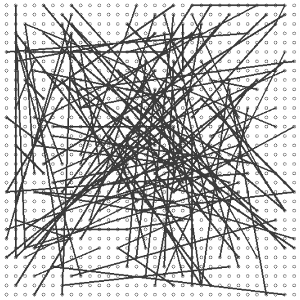
\includegraphics[width=\linewidth]{images/feature/brief.png}
    \caption{BRIEF Descriptor~\cite{Calonder2012}}
  \end{subfigure}
  \begin{subfigure}[t]{0.33\textwidth}
    \centering
    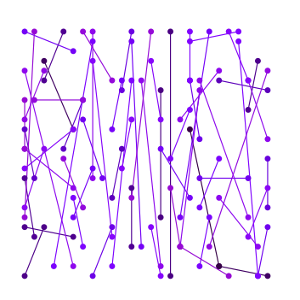
\includegraphics[width=\linewidth]{images/feature/orb.png}
    \caption{ORB Descriptor~\cite{Rublee2011}}
  \end{subfigure}
  \begin{subfigure}[t]{0.31\textwidth}
    \centering
    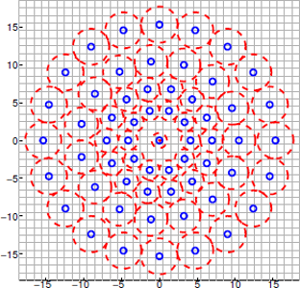
\includegraphics[width=\linewidth]{images/feature/brisk.png}
    \caption{BRISK Descriptor~\cite{Leutenegger2011}}
  \end{subfigure}
  \caption{Binary Descriptors}
  \label{fig:binary_descriptors}
\end{figure}

% \begin{figure}[htp]
% 	\centering
% 	\begin{subfigure}[t]{0.45\textwidth}
% 		\centering
% 		\includegraphics[width=\linewidth]{images/background/orb_matches1.png}
% 	\end{subfigure}
% 	\hspace{1.0em}
% 	\begin{subfigure}[t]{0.45\textwidth}
% 		\centering
% 		\includegraphics[width=\linewidth]{images/background/orb_matches2.png}
% 	\end{subfigure}
% 	\caption{ORB descriptors detecting features in the EuRoC MAV dataset~\cite{Burri2016}}
% 	\label{fig:orb_descriptors_in_action}
% \end{figure}
%
% Following~\cite{Shelly2014}, the ORB descriptor was chosen for experimentation.
% The ORB descriptor is considered as an improvement over BRIEF with the addition
% of being orientation invariant. However, it can be observed in
% Fig.~\ref{fig:orb_descriptors_in_action} that the ORB detector from OpenCV
% strongly favours strong corners over keeping the detected points uniform over
% the image space. As a result the key-points are mostly clustered around the
% chessboard observed in the scene. This is in contrast to Grid-FAST discussed in
% Section.~\ref{subsec:fast_feature_detection}, where the features detected are
% uniformly distributed over the entire image space. Because of ORB features not
% being uniformly distributed, the KLT feature tracker is considered and is
% discussed in the following section.



\section{KLT Feature Tracker}
\label{sec:klt}

In the previous section, we showed how ORB descriptors and matching methods are
used to correspond and match features across multiple camera frames. This
process of corresponding the the same features across multiple camera frames is
called feature tracking. There are many different feature tracking pipelines.
Matching feature descriptors such as ORB has shown to have better temporal
tracking accuracy compared to KLT-based methods~\cite{Paul2017}. However, in
the work of~\cite{Sun2018}, descriptor-based feature trackers were found to
require more computational resources with limited gains in tracking accuracy.
Making it less attractive for real-time operation. In the following we will
briefly describe the KLT feature tracker, but first an understanding of optical
flow is required.


\subsubsection{Optical Flow}

Optical flow estimates the velocity of each image feature in successive images
of a scene. It makes the following explicit assumptions:

\begin{itemize}
  \setlength{\itemsep}{1pt}
  \setlength{\parskip}{0pt}
  \setlength{\parsep}{0pt}

  \item{Pixel intensity does not change between consecutive frames}
  \item{Displacement of features is small}
  \item{Features are within the same local neighbourhood}
\end{itemize}

Let us consider a pixel, $p$, in the first frame which has an intensity, $I(x,
y, t)$, where it is a function of the pixel location, $x$ and $y$, and time,
$t$. If we apply the aforementioned assumptions, we can say that the intensity
of said pixel in the first frame to the second does not change. Additionally,
if there was a small displacement, $dx$ and $dy$, and small time difference,
$dt$, between images this can be written in mathematical form as,
%
\begin{equation}
  \label{eq:brightness_constancy}
  I(x, y, t) = I(x + dx, y + dy, t + dt).
\end{equation}
%
This is known as the brightness constancy equation. To obtain the image
gradient and velocity of the pixel, we can use Taylor series approximation of
right-hand side of Eq.~\eqref{eq:brightness_constancy} to get,
%
\begin{equation}
  I(x + dx, y + dy, t + dt) = I(x, y, t)
    + \dfrac{\partial{I}}{\partial{x}} dx
    + \dfrac{\partial{I}}{\partial{y}} dy
    + \dfrac{\partial{I}}{\partial{t}} dt
    + \text{H.O.T},
\end{equation}
%
removing common terms and dividing by $dt$ we get,
%
\begin{equation}
  \label{eq:optical_flow}
  I_{x} v_{x} + I_{y} v_y + I_{t} = 0
\end{equation}
or,
%
\begin{equation}
  \label{eq:optical_flow_2}
  I_{x} v_{x} + I_{y} v_y = -I_{t}
\end{equation}
%
where:
%
\begin{align}
  I_{x} = \dfrac{\partial I}{\partial x}
  ; \quad
  I_{y} = \dfrac{\partial I}{\partial y} \nonumber \\
  v_{x} = \dfrac{dx}{dt}
  ; \quad
  v_y = \dfrac{dy}{dt}. \nonumber
\end{align}
%
The image gradients along the x and y directions are $I_{x}$ and $I_{y}$, where
$I_{t}$ is the image gradient along time, finally, $v_{x}$ and $v_{y}$ are the
pixel velocity in $x$ and $y$ directions, which is unknown. The problem with
Eq.~\ref{eq:optical_flow_2} is that it provides a single constraint with two
degrees of freedom, and as such requires at least one additional constraint to
identify a solution.

The Lucas-Kanade method solves the aperture problem by introducing additional
conditions. This method assumes all pixels within a window centered around a
pixel $p$ will have similar motion, and that the window size is configurable.
For example, a window size of $3 \times 3$ around the pixel $p$, the $9$ points
within the window should have a similar motion. Using
Eq.~\ref{eq:optical_flow_2}, the intensity inside the window must therefore
satisfy,
%
\begin{align}
  I_{x}(p_1) v_{x}(p_1) &+ I_{y}(p_1) v_y = -I_{t}(p_1) \nonumber \\
  I_{x}(p_1) v_{x}(p_2) &+ I_{y}(p_2) v_y = -I_{t}(p_2) \nonumber \\
  & \enspace \vdots \nonumber \\
  I_{x}(p_1) v_{x}(p_n) &+ I_{y}(p_n) v_y = -I_{t}(p_n) \nonumber
\end{align}
%
where $p_{1}, p_{2} ,\dots , p_{n}$ are the pixels in the window. This can be
re-written in matrix form $\mathbf{A} \mathbf{x} = \mathbf{b}$ as,
%
\begin{equation}
  \label{eq:lucas_kanade_1}
    \mathbf{A} = \begin{bmatrix}
        I_{x}(p_{1}) & I_{y}(p_{1}) \\
        I_{x}(p_{2}) & I_{y}(p_{2}) \\
        \vdots & \vdots \\
        I_{x}(p_{n}) & I_{y}(p_{n})
    \end{bmatrix}
    \quad
    \mathbf{x} = \begin{bmatrix}
      v_{x} \\ v_{y} \\
    \end{bmatrix}
    \quad
    \mathbf{b} = \begin{bmatrix}
      -I_{t}(p_{1}) \\
      -I_{t}(p_{2}) \\
      \vdots \\
      -I_{t}(p_{n})
    \end{bmatrix}.
\end{equation}
%
The linear system of equations of Eq.~\ref{eq:lucas_kanade_1} is
over-determined, therefore there is no exact solution. To address this issue, a
least squares method can be used to approximate the solution by applying the
ordinary least squares. For the system $\mathbf{A} \mathbf{x} = \mathbf{b}$,
the least squares formula is obtained by minimizing the following,
%
\begin{equation}
  \underset{\mathbf{x}}{\text{argmin }} || \mathbf{A} \mathbf{x} - \mathbf{b} ||,
\end{equation}
%
the solution of which can be obtained by using \textit{normal equations},
%
\begin{align}
  \label{eq:normal_equations_1}
  \mathbf{A}^{T} \mathbf{A} \mathbf{x} &= \mathbf{A}^{T} \mathbf{b} \\
  \label{eq:normal_equations_2}
  \mathbf{x} &= (\mathbf{A}^{T} \mathbf{A})^{-1} \mathbf{A}^{T} \mathbf{b}.
\end{align}
%
Rewriting Eq~\ref{eq:lucas_kanade_1} in the form of Eq.~\ref{eq:normal_equations_2} we get,
%
\begin{equation}
  \begin{bmatrix}
  v_{x} \\ v_{y}
  \end{bmatrix}
  =
  \begin{bmatrix}
    \sum_{i}{I_{x}(p_{i})}^2 & \sum_{i}{I_{x}(p_{i}) I_{y}(p_{i}) } \\ 
    \sum_{i}{I_{x}(p_{i}) I_{y}(p_{i})} & \sum_{i}{I_{y}(p_{i})}^2
  \end{bmatrix}^{-1}
  \begin{bmatrix}
    - \sum_{i}{I_{x}(p_{i}) I_{t}(p_{i})} \\ 
    - \sum_{i}{I_{y}(p_{i}) I_{t}(p_{i})}
  \end{bmatrix}
\end{equation}
%
which is finally used to obtain the optical flow of pixel $p$.

% \begin{figure}[H]
% 	\centering
% 	\begin{subfigure}[t]{0.47\textwidth}
% 		\centering
% 		\includegraphics[width=\linewidth]{images/background/klt_matches1.png}
% 	\end{subfigure}
% 	\hspace{1.0em}
% 	\begin{subfigure}[t]{0.47\textwidth}
% 		\centering
% 		\includegraphics[width=\linewidth]{images/background/klt_matches2.png}
% 	\end{subfigure}
% 	\caption{KLT Feature Tracker in Action}
% 	\label{fig:klt_in_action}
% \end{figure}


\subsubsection{KLT Feature Tracker}

The Lucas-Kanade method recovers feature pixel velocities from consecutive
camera frames. The issue with the Lucas-Kanade method is that it assumes the
features detected have small displacements between consecutive camera frames.
Therefore to track features that have a large motion the Kanade-Lucas-Tomasi
(KLT) feature tracker~\cite{Lucas1981} uses reduced-scale versions of the input
images in order to track features over multiple camera frames. The general
steps of the KLT feature tracker is as follows,
%
\begin{enumerate}
	\item{Detect corners in the first camera frame}
	\item{For each corners, compute the motion between consecutive camera frames
			  using a pyramidal implementation of the Lucas-Kanade method}
	\item{Match motion vectors between consecutive camera frames to track corners}
	\item{Detect new corners if number of tracks currently tracking is too low}
	\item{Repeat steps 2 to 4}
\end{enumerate}

\chapter{Rotations}

\section{Euler Angles}
Z-Y-X rotation sequence:

\begin{equation}
  \rot_{zyx} =
  \begin{bmatrix}
    c(\psi) c(\theta)
    & c(\psi) s(\theta) s(\phi) - s(\psi) c(\phi)
    & c(\psi) s(\theta) c(\phi) + s(\psi) s(\phi) \\
    s(\psi) c(\theta)
    & s(\psi) s(\theta) s(\phi) + c(\psi) c(\phi)
    & s(\psi) s(\theta) c(\phi) - c(\psi) s(\phi) \\
    -s(\theta) & c(\theta) s(\phi) & c(\theta) c(\phi)
  \end{bmatrix}
\end{equation}



% QUATERNIONS
\section{Quaternions}

A quaternion, $\Vec{q} \in \real^{4}$, generally has the following form
%
\begin{equation}
  \quat = q_{w} + q_{x} \mathbf{i} + q_{y} \mathbf{j} + q_{z} \mathbf{k},
\end{equation}
%
where $\{ q_{w}, q_{x}, q_{y}, q_{z} \} \in \real$ and $\{ \mathbf{i}, \mathbf{j},
\mathbf{k} \}$ are the imaginary numbers satisfying
%
\begin{equation}
\begin{split}
  &\mathbf{i}^{2}
  = \mathbf{j}^{2}
  = \mathbf{k}^{2}
  = \mathbf{ijk}
  = -1 \\
  \mathbf{ij} = -\mathbf{ji} &= \mathbf{k}, \enspace
  \mathbf{jk} = -\mathbf{kj} = \mathbf{i}, \enspace
  \mathbf{ki} = -\mathbf{ik} = \mathbf{j}
\end{split}
\end{equation}
%
corresponding to the Hamiltonian convention. The quaternion can be written as a
4 element vector consisting of a \textit{real} (\textit{scalar}) part, $q_{w}$,
and \textit{imaginary} (\textit{vector}) part $\quat_{v}$ as,
%
\begin{equation}
  \quat =
  \begin{bmatrix} q_{w} \\ \quat_{v} \end{bmatrix} =
  \begin{bmatrix} q_{w} \\ q_{x} \\ q_{y} \\ q_{z} \end{bmatrix}
\end{equation}
%
There are other quaternion conventions, for example, the JPL convention. A more
detailed discussion between Hamiltonian and JPL quaternion convention is
discussed in \cite{Sola2017}.


\subsection{Main Quaternion Properties}
\subsubsection{Sum}

Let $\Vec{p}$ and $\Vec{q}$ be two quaternions, the sum of both quaternions is,
%
\begin{equation}
  \Vec{p} \pm \Vec{q} =
  \begin{bmatrix} p_w \\ \Vec{p}_{v} \end{bmatrix}
  \pm
  \begin{bmatrix} q_w \\ \Vec{q}_{v} \end{bmatrix} =
  \begin{bmatrix} p_w \pm q_w \\ \Vec{p}_{v} \pm \Vec{q}_{v} \end{bmatrix}.
\end{equation}
%
The sum between two quaternions $\Vec{p}$ and $\Vec{q}$ is \textbf{commutative}
and \textbf{associative}.
%
\begin{equation}
  \Vec{p} + \Vec{q} = \Vec{q} + \Vec{p}
\end{equation}
%
\begin{equation}
  \Vec{p} + (\Vec{q} + \Vec{r}) = (\Vec{p} + \Vec{q}) + \Vec{r}
\end{equation}


\subsubsection{Product}

The quaternion multiplication (or product) of two quaternions $\Vec{p}$ and
$\Vec{q}$, denoted by $\otimes$ is defined as
%
\begin{align}
  \Vec{p} \otimes \Vec{q}
    &=
    (p_w + p_x \mathbf{i} + p_y \mathbf{j} + p_z \mathbf{k})
    (q_w + q_x \mathbf{i} + q_y \mathbf{j} + q_z \mathbf{k}) \\
    &=
    \begin{matrix}
      &(p_w q_w - p_x q_x - p_y q_y - p_z q_z)& \\
      &(p_w q_x + p_x q_w + p_y q_z - p_z q_y)& \mathbf{i}\\
      &(p_w q_y - p_y q_w + p_z q_x + p_x q_z)& \mathbf{j}\\
      &(p_w q_z + p_z q_w - p_x q_y + p_y q_x)& \mathbf{k}\\
    \end{matrix} \\
    &=
    \begin{bmatrix}
      \label{eq:quaternion_product}
      p_w q_w - p_x q_x - p_y q_y - p_z q_z \\
      p_w q_x + q_x p_w + p_y q_z - p_z q_y \\
      p_w q_y - p_y q_w + p_z q_x + p_x q_z \\
      p_w q_z + p_z q_w - p_x q_y + p_y q_x \\
    \end{bmatrix} \\
    &=
    \begin{bmatrix}
      \label{eq:quaternion_product_2}
      p_w q_w - \Transpose{\Vec{p}_{v}} \Vec{q}_{v} \\
      p_w \Vec{q}_{v} + q_w \Vec{p}_{v} + \Vec{p}_{v} \times \Vec{q}_{v}
    \end{bmatrix}.
\end{align}
%
The quaternion product is \textbf{not commutative} in the general
case\footnote{There are exceptions to the general non-commutative rule, where
either $\Vec{p}$ or $\Vec{q}$ is real such that $\Vec{p}_{v} \times \Vec{q}_{v}
= 0$, or when both $\Vec{p}_v$ and $\Vec{q}_v$ are parallel, $\Vec{p}_v ||
\Vec{q}_v$. Only in these cirmcumstances is the quaternion product
commutative.},
%
\begin{equation}
  {\Vec{p} \otimes \Vec{q} \neq \Vec{q} \otimes \Vec{p}} \enspace .
\end{equation}
%
The quaternion product is however \textbf{associative},
%
\begin{equation}
  \Vec{p} \otimes (\Vec{q} \otimes \Vec{r})
  = (\Vec{p} \otimes \Vec{q}) \otimes \Vec{r}
\end{equation}
%
and \textbf{distributive over the sum}
%
\begin{equation}
  \Vec{p} \otimes (\Vec{q} + \Vec{r}) =
  \Vec{p} \otimes \Vec{q} + \Vec{p} \otimes \Vec{r}
  \quad \text{and} \quad
  (\Vec{p} \otimes \Vec{q}) + \Vec{r} =
  \Vec{p} \otimes \Vec{r} + \Vec{q} \otimes \Vec{r}
\end{equation}

The quaternion product can alternatively be expressed in matrix form as
%
\begin{equation}
  \Vec{p} \otimes \Vec{q} = [\Vec{p}]_{L} \Vec{q}
  \quad \text{and} \quad
  \Vec{p} \otimes \Vec{q} = [\Vec{q}]_{R} \Vec{p} \enspace ,
\end{equation}
%
where $[\Vec{p}]_{L}$ and $[\Vec{q}]_{R}$ are the left and right
quaternion-product matrices which are derived from
\eqref{eq:quaternion_product},
%
\begin{equation}
  [\Vec{p}]_{L} =
  \begin{bmatrix}
    p_w & -p_x & -p_y & -p_z \\
    p_x & p_w & -p_z & p_y \\
    p_y & p_z & p_w & -p_x \\
    p_z & -p_y & p_x & p_w
  \end{bmatrix},
  \quad \text{and} \quad
  [\Vec{q}]_{R} =
  \begin{bmatrix}
    q_w & -q_x & -q_y & -q_z \\
    q_x & q_w & q_z & -q_y \\
    q_y & -q_z & q_w & q_x \\
    q_z & q_y & -q_x & q_w
  \end{bmatrix},
\end{equation}
%
or inspecting \eqref{eq:quaternion_product_2} a compact form can be derived as,
%
\begin{equation}
  [\Vec{p}]_{L} =
  \begin{bmatrix}
    0 & -\Transpose{\Vec{p}_{v}} \\
    \Vec{p}_w \I_{3 \times 3} + \Vec{p}_{v} &
    \Vec{p}_w \I_{3 \times 3} -\Skew{\Vec{p}_{v}}
  \end{bmatrix}
\end{equation}
%
and
%
\begin{equation}
  [\Vec{q}]_{R} =
  \begin{bmatrix}
    0 & -\Transpose{\Vec{q}_{v}} \\
    \Vec{q}_w \I_{3 \times 3} + \Vec{q}_{v} &
    \Vec{q}_w \I_{3 \times 3} -\Skew{\Vec{q}_{v}}
  \end{bmatrix},
\end{equation}
%
where $\Skew{\bullet}$ is the skew operator that produces a matrix cross
product matrix, and is defined as
%
\begin{equation}
  \Skew{\Vec{v}} =
  \begin{bmatrix}
    0 & -v_{3} & v_{2} \\
    v_{3} & 0 & -v_{1} \\
    -v_{2} & v_{1} & 0
  \end{bmatrix},
  \quad
  \Vec{v} \in \real^{3}
\end{equation}
%

\subsubsection{Conjugate}

The conjugate operator for quaternion, ${(\bullet)}^{\ast}$, is
defined as
%
\begin{equation}
  \quat^{\ast}
  =
  \begin{bmatrix}
    q_w \\
    - \Vec{q}_v
  \end{bmatrix}
  =
  \begin{bmatrix}
    q_w \\
    - q_x \\
    - q_y \\
    - q_z
  \end{bmatrix}.
\end{equation}
%
This has the properties
%
\begin{equation}
  \quat \otimes \quat^{-1}
  = \quat^{-1} \otimes \quat
  = q_{w}^{2} + q_{x}^{2} + q_{y}^{2} + q_{z}^{2}
  =
  \begin{bmatrix}
    q_{w}^{2} + q_{x}^{2} + q_{y}^{2} + q_{z}^{2} \\
    \Vec{0}
  \end{bmatrix},
\end{equation}
%
and
%
\begin{equation}
  (\Vec{p} \otimes \Vec{q})^{\ast}
  = \Vec{q}^{\ast} \otimes \Vec{p}^{\ast}.
\end{equation}


\subsubsection{Norm}

The norm of a quaternion is defined by
%
\begin{align}
  \Norm{\quat} &= \sqrt{\quat \otimes \quat^{\ast}} \\
    &= \sqrt{\quat^{\ast} \otimes \quat} \\
    &= \sqrt{q_{w}^{2} + q_{x}^{2} + q_{y}^{2} + q_{z}^{2}}
    \enspace \in \real,
\end{align}
%
and has the property
%
\begin{align}
  \Norm{\Vec{p} \otimes \Vec{q}} =
  \Norm{\Vec{q} \otimes \Vec{p}} =
  \Norm{\Vec{p}} \Norm{\Vec{q}}
\end{align}



% -- QUATERNION FROM TWO VECTORS
\subsection{Quaternion from Two Vectors}

% TODO: Need to reword the beginning
Using the properties of the cross and dot product
%
\begin{align}
  \Vec{u} \cdot \Vec{v} &=
    \Norm{\Vec{u}} \Norm{\Vec{v}} \cos \theta \\
  \Norm{\Vec{u} \times \Vec{v}} &=
    \Norm{\Vec{u}} \Norm{\Vec{v}} \Norm{\sin \theta} ,
\end{align}
%
the axis angle, $\boldsymbol{\theta} \in \real^{3}$, can be obtained from
$\Vec{u}$ and $\Vec{v}$ with
%
\begin{align}
  % -- Axis-angle
  \boldsymbol{\theta} &= \theta \Vec{e} \\
  % -- Angle
  \label{eq:angle_axis_calc_angle}
  \theta &= \cos^{-1}(
    \dfrac{\Vec{u} \cdot \Vec{v}}
          {\Norm{\Vec{u}} \Norm{\Vec{v}}}
  ) \quad , \enspace \theta \in \real \\
  % -- Axis
  \label{eq:angle_axis_calc_axis}
  \Vec{e} &=
    \dfrac{\Vec{u} \times \Vec{v}}{\Norm{\Vec{u} \times \Vec{v}}}
    \quad , \enspace \Vec{e} \in \real^{3}
\end{align}
%
where $\Vec{e}$ is the unit vector that defines the rotation axis and $\theta$
is the rotation angle about $\Vec{e}$. Once the axis angle,
$\boldsymbol{\theta}$, is obtained a quaternion can be formed
%
\begin{equation}
  \label{eq:quaternion_from_axis_angles}
  \quat =
    \cos \dfrac{\theta}{2}
    + \Vec{i} \sin \dfrac{\theta}{2} e_{x}
    + \Vec{j} \sin \dfrac{\theta}{2} e_{y}
    + \Vec{k} \sin \dfrac{\theta}{2} e_{z} \enspace .
\end{equation}


\subsubsection{Example: Attitude from gravity and accelerometer vectors}

In robotics knowing the attitude of the system is often required. An Inertial
Measurement Unit (IMU) is commonly used to obtain this information. Using the
method described previously, a gravity vector along with an accelerometer
measurement vector can be used to obtain an attitude in form of a quaternion.

Let $\Vec{g} \in \real^{3}$ be the gravity vector, and $\Vec{a}_{m} \in
\real^{3}$ be the accelerometer measurement from an IMU. With the two vectors
$\Vec{g}$ and $\Vec{a}_{m}$ a quaternion $\quat_{\world\sensor}$ expressing the
rotation of the IMU sensor frame, $\frame_{\sensor}$, with respect to the world
frame, $\frame_{\world}$, can be calculated given that values for $\Vec{g}$ and
$\Vec{a}_{m}$ are known. For example let
%
\begin{align}
  % -- Gravity vector
  \Vec{g} &= \Transpose{\begin{bmatrix} 0 & 0 & -9.81 \end{bmatrix}} \\
  % -- Accelerometer measurement vector
  \Vec{a}_{m} &= \Transpose{
    \begin{bmatrix}
      9.2681 &
      -0.310816 &
      -3.14984
    \end{bmatrix}
  } ,
\end{align}
%
taken from the first measurement of the \texttt{imu\_april} calibration
sequence of the EuRoC MAV dataset.

\begin{figure}[htp]
  \centering
  \begin{subfigure}[b]{0.47\textwidth}
    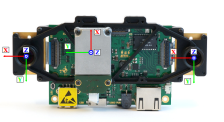
\includegraphics{images/quaternion/visensor_frames}
    \caption{VI-Sensor Coordinate Frames}
  \end{subfigure}
  ~ \quad
  \begin{subfigure}[b]{0.47\textwidth}
    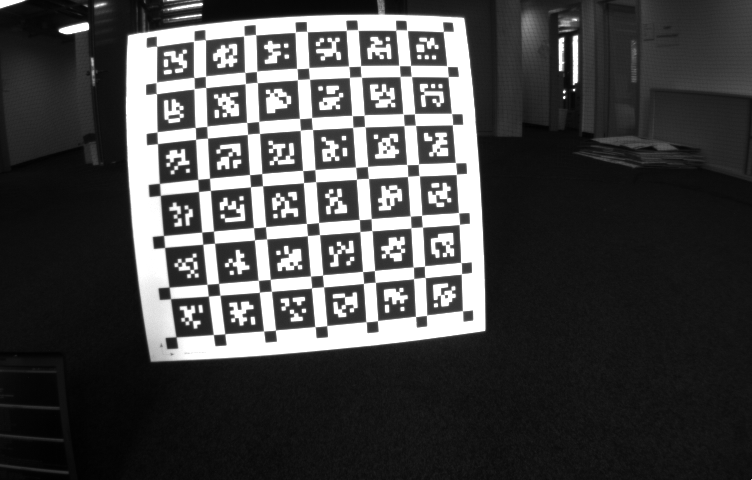
\includegraphics[width=\textwidth]{images/quaternion/1404733405732800000}
    \caption{Image frame}
  \end{subfigure}
  % \caption{EuRoC MAV Dataset - \begin{verbatim}imu_april\end{verbatim} sequence}
  \caption{EuRoC MAV Dataset - \texttt{imu\_april} Sequence}
\end{figure}

Before calculating the axis-angle, however, it should be noted that when an
accelerometer is at rest the measurement reading in the z-axis is positive
instead of negative. The reason is accelerometers measures acceleration by
measuring the displacement of a proof mass that is suspended with springs. For
example, if gravity is ignored and the accelerometer moves upwards, the proof mass
will be displaced towards the bottom of the accelerometer. This is interpreted
as an acceleration in the upwards direction, and so when the accelerometer is
at rest on a flat surface, gravity pulls on the proof mass yeilding a positive
measurement in the upwards direction. To resolve this issue the gravity vector
is negated, and so $\Vec{u} = -\Vec{g}$ and $\Vec{v} = \Vec{a}_{m}$. Using 
\eqref{eq:angle_axis_calc_angle} and \eqref{eq:angle_axis_calc_axis} the
axis-angle, $\boldsymbol{\theta}$, is thereby
%
\begin{align}
  % -- Axis-Angle
  \theta &= 1.8982 \\
  \Vec{e} &= \Transpose{
    \begin{bmatrix}
      0.03352 &
      0.99944 &
      0.00000
    \end{bmatrix}
  }
\end{align}
%
Finally the quaternion, $\quat_{\world\sensor}$, can be calculated using
\eqref{eq:quaternion_from_axis_angles} resulting in
%
\begin{equation}
  % -- Quaternion
  \quat_{\world\sensor} &= \Transpose{
    \begin{bmatrix}
      0.58240 &
      0.02725 &
      0.81245 &
      0.00000
    \end{bmatrix}
  } \enspace .
\end{equation}



% -- QUATERNION TO ROTATION MATRIX
\subsection{Quaternion to Rotation Matrix}

\begin{equation}
  \Mat{R}\{\quat \} = \begin{bmatrix}
    q_w^2 + q_x^2 - q_y^2 - q_z^2
    & 2(q_x q_y - q_w q_z)
    & 2(q_x q_z + q_w q_y) \\
    2(q_x q_y + q_w q_z)
    & q_w^2 - q_x^2 + q_y^2 - q_z^2
    & 2(q_y q_z - q_w q_x) \\
    2(q_x q_y - q_w q_y)
    & 2(q_y q_z + q_w q_x)
    & q_w^2 - q_x^2 - q_y^2 + q_z^2
  \end{bmatrix}
\end{equation}



% -- ROTATION MATRIX TO QUATERNION
\subsection{Rotation Matrix to Quaternion}

\begin{align}
  q_w &= \dfrac{\sqrt{1 + m_{11} + m_{22} + m_{33}}}{2} \\
  q_x &= \dfrac{m_{32} - m_{23}}{4 q_w} \\
  q_y &= \dfrac{m_{13} - m_{31}}{4 q_w} \\
  q_z &= \dfrac{m_{21} - m_{02}}{4 q_w}
\end{align}

Note, while the equations seems straight forward in practice, however,the trace
of the rotation matrix need to be checked inorder to guarantee correctness.




% DIFFERENTIAL CALCULUS OF 3D CALCULUS
\section{Differential Calculus}

Lie Group $SO(3)$
\begin{itemize}
  \item{Not a vector space}
  \item{Has no addition operator
  \item{Has no subtraction operator
\end{itemize}

State estimation frameworks rely on small differences and gradients in order to
correct the state estimate. Orientations unlike translation and velocity do not
have an addition operator, as such it is more involving to update or
find the gradients of orientations. Forunately, since orientations are a
special orhogonal group $SO(3)$ as well as a Lie group, an exponential map
exists that relates to its Lie algebra allowing orientations to be perturbed
and its gradients calculated.

Elements in Lie algebra are abstract vectors and not suitable for actual
computations. A basis $\mathbf{B} = [\vec{\boldsymbol{\varphi}}_{1} \enspace
\vec{\boldsymbol{\varphi}}_{2} \enspace \vec{\boldsymbol{\varphi}}_{3}]$
can be used to extend the map to $\real^{3}$. 

The definition of an exponential map $\text{exp} : \real^{3} \mapsto SO(3)$ of a
coordinate tuple $\boldsymbol{\varphi} (\varphi_1, \varphi_2, \varphi_3) \in
\real^{3}$ is defined by

\begin{equation}
  \text{exp}(\boldsymbol{\varphi}) := Exp(
    \vec{\boldsymbol{\varphi}}_{1}\varphi_{1},
    \vec{\boldsymbol{\varphi}}_{2}\varphi_{2},
    \vec{\boldsymbol{\varphi}}_{3}\varphi_{3}
  )
\end{equation}


$\forall t, s \in \real$, $\forall \vec{\boldsymbol{\varphi}} \in $

\begin{align}
  Exp((t + s) \vec{\boldsymbol{\varphi}}) =
    Exp(t\vec{\boldsymbol{\varphi}}) \circ Exp(s\vec{\boldsymbol{\varphi}})
\end{align}


\begin{align}
  \boxplus :& SO(3) \times \real^{3} \rightarrow SO(3), \\
    &\Phi, \boldsymbol{\varphi}
      \mapsto \text{exp}(\boldsymbol{\varphi}) \circ \Phi, \nonumber \\
  \boxminus :& SO(3) \times SO(3) \rightarrow \real^{3}, \\
    &\Phi_1, \Phi_2 \mapsto \text{log}(\Phi_1 \circ \Phi_{2}^{-1}) \nonumber
\end{align}

Similar to regular addition and subtraction, both operators have the following
identities,
%
\begin{align}
  \Phi \boxplus \Vec{0} &= \Phi \\
  (\Phi \boxplus \boldsymbol{\varphi}) \boxminus \Phi &= \boldsymbol{\varphi} \\
  \Phi_1 \boxplus (\Phi_2 \boxminus \Phi_1) &= \Phi_2
\end{align}

\chapter{Optimization}

\section{Linear Least Squares}

Linear problems generally have the form
%
\begin{equation}
  \Mat{A} \Vec{x} = \Vec{b}
\end{equation}
%
If $\Mat{A}$ is skinny (number of rows is larger than number of columns) the
problem is over constrained and there is no \textit{unique} solution. Instead,
the problem can be solved by minizming the squared error between $\Mat{A}
\Vec{x}$ and $\Vec{b}$. The linear least squares problem is then defined as,
%
\begin{equation}
  &\min_{\Vec{x}} || \Mat{A} \Vec{x} - \Vec{b} ||^{2}_{2} \enspace,
\end{equation}
%
where the goal is to find an \textit{approximate} solution.

The local minima can be found when the derivative of the squared error is zero.
First the squared error is expanded to give:
%
\begin{align}
  & (\Mat{A} \Vec{x} - \Vec{b})^{\transpose}
    (\Mat{A} \Vec{x} - \Vec{b}) \\
  & (\Transpose{\Vec{x}} \Transpose{\Mat{A}} \Mat{A} \Vec{x}
    - 2 \Transpose{\Vec{b}} \Mat{A} \Vec{x}
    + \Transpose{\Vec{b}} \Vec{b})
\end{align}
%
then by differentiating the expanded squared error with respect to $\Vec{x}$,
setting the derivative to zero, and rearranging the equation with respect to
$\Vec{x}$ gives the following
%
\begin{align}
  % Line 1
  2 \Transpose{\Vec{x}} \Transpose{\Mat{A}} \Mat{A}
    - 2 \Transpose{\Vec{b}} \Mat{A} &= 0 \\
  % Line 2
  \Transpose{\Vec{x}} \Transpose{\Mat{A}} \Mat{A}
    &= \Transpose{\Vec{b}} \Mat{A} \\
  % Line 3
  \Transpose{\Mat{A}} \Mat{A} \Vec{x}
    &= \Transpose{\Mat{A}} \Vec{b} \\
  % Line 4
  \Vec{x}
    &= \left( \Transpose{\Mat{A}} \Mat{A} \right)^{-1}
      \Transpose{\Mat{A}} \Vec{b} \\
  % Line 5
  \Vec{x}
    &= \Mat{A}^{\dagger} \Vec{b} \enspace,
\end{align}
%
where $\left( \Transpose{\Mat{A}} \Mat{A} \right)^{-1} \Transpose{\Mat{A}}$ is
known as the pseudo inverse $\Mat{A}^{\dagger}$.



\section{Non-linear Least Squares}

A non-linear least squares is an optimization problem that minimizes the sum of
squares of the residual functions, and has the form
%
\begin{equation}
  \min_{\Vec{x}} \enspace
    \dfrac{1}{2}
    \Vec{e}(\Vec{x})^{\transpose}
    \Mat{W} \,
    \Vec{e}(\Vec{x})
\end{equation}
%
where the error function, $\Vec{e}(\cdot)$, depends on the optimization
parameter, $\Vec{x} \in \real^{n}$. The error function, $\Vec{e}(\cdot)$, has a
form of
%
\begin{equation}
  \Vec{e}_{i} =
    \Vec{z} - \Vec{h}(\Vec{x})
\end{equation}
%
is defined as the difference between the measured value, $\Vec{z}$, and the
estimated value calculated using the measurement function, $\Vec{h}(\cdot)$.

A local minima for the problem is found when the gradient of the cost,
$\Vec{C}$, is zero
%
\begin{align}
  \dfrac{\partial{\Vec{C}}}{\partial{\Vec{x}}}
  &=
    \dfrac{\partial{\Vec{C}}}{\partial{\Vec{e}}}
    \dfrac{\partial{\Vec{e}}}{\partial{\Vec{x}}} \\
  &=
    \Vec{e}(\Vec{x})^{\transpose}
    \Mat{W}
    \dfrac{\partial{\Vec{e}}}{\partial{\Vec{x}}} \\
  &=
    \Vec{e}(\Vec{x})^{\transpose}
    \Mat{W}
    \Vec{E}(\Vec{x})
\end{align}
%
linearizing $\Vec{e}(\Vec{x})$ with the first-order Taylor series,
$\Vec{e}(\Vec{x}) \approx \Vec{e}(\bar{\Vec{x}}) + \Vec{E}(\bar{\Vec{x}})
\Delta\Vec{x}$, gives,
%
\begin{align}
  \dfrac{\partial{\Vec{C}}}{\partial{\Vec{x}}}
  &=
    (\Vec{e}(\bar{\Vec{x}}) + \Vec{E}(\bar{\Vec{x}})\Delta\Vec{x})^{\transpose}
    \Mat{W} \Vec{E}(\Vec{x})
  = 0 \\
  &\Vec{e}(\bar{\Vec{x}})^{\transpose} \Mat{W} \Vec{E}(\bar{\Vec{x}})
    + \Delta\Vec{x}^{\transpose} \Vec{E}(\bar{\Vec{x}})^{\transpose}
      \Mat{W}
      \Vec{E}(\bar{\Vec{x}})
    = 0 \\
  &\Vec{E}(\bar{\Vec{x}})^{\transpose} \Mat{W} \, \Vec{e}(\bar{\Vec{x}})
    + \Vec{E}(\bar{\Vec{x}})^{\transpose}
      \Mat{W}
      \Vec{E}(\bar{\Vec{x}})
      \Delta\Vec{x}
    = 0 \\
  &\underbrace{
      \Vec{E}(\bar{\Vec{x}})^{\transpose}
      \Mat{W}
      \Vec{E}(\bar{\Vec{x}})
  }_{\Mat{A}}
  \underbrace{
    \vphantom{
      \Vec{E}(\bar{\Vec{x}})^{\transpose}
      \Mat{W}
      \Vec{E}(\bar{\Vec{x}})
    }
    \Delta\Vec{x}
  }_{\Vec{x}}
  =
  \underbrace{
    - \Vec{E}(\bar{\Vec{x}})^{\transpose}
    \Mat{W} \,
    \Vec{e}(\bar{\Vec{x}})
  }_{\Vec{b}}
\end{align}
%
solve the normal equations for $\Delta\Vec{x}$ and update $\Vec{x}$ using,
%
\begin{equation}
  \Vec{x}^{k+1} = \Vec{x}^{k} + \Delta{\Vec{x}}
\end{equation}



\section{Gauge}

Gauge theory is borrowed from physics.

Accurate structure from motion or vision based state estimation is hard. One
hurdle is addressing the accuracy quantitatively. There are two main problems
that arise:

\begin{itemize}
  \item{\textbf{Inherent Physical Indeterminancy}: cause by loss of information
    while projecting 3D objects onto a 2D image plane.}
  \item{\textbf{Overparameterized Problem}: e.g. a shape model that can be
    parameterized by a vector, each representing the absolute position and
    orientation of the object could itself be indeterminant.}
\end{itemize}

It is well known that a vision only bundle adjustment has 7 unobserable
degrees-of-freedom (DoF), while for a VI-system, the global position and global
yaw is not observable, a total of four unobservable DoFs. These unobservable
DoFs (a.k.a gauge freedoms) have to be handled properly.

There are three main approaches to address the unobservability in a VI-system.
They are \textit{gauge fixation}, \textit{gauge prior}, \textit{free gauge}.


\subsection{Gauge fixation}

Gauge fixation method works by decreasing the number of optimization parameters to
where there are no unobservable states left for the opitmization problem to
optimize. This is to ensure the Hessian is well conditioned and invertable.
This approach enforces hard constraints to the solution.

The standard method to update orientation variables such as a rotation,
$\rot$, during the iterations of a non-linear least squares solver is to use
local coordinates, where at the $k$-th iteration, the update is
%
\begin{equation}
  \label{eq:opt-rot_std_update}
  \rot^{k + 1} = \text{Exp}(\delta \boldsymbol{\phi}^{k}) \rot^{k} .
\end{equation}

Setting the $z$ component of $\boldsymbol{\phi}^{k}$ to 0 allows fixating the
yaw with respect to $\rot^{k}$. However, concatenating several such updates
over $K$-iterations,
%
\begin{equation}
  \rot^{K} = \prod^{K-1}_{k=0} \text{Exp}(\delta \boldsymbol{\phi}^{k}) ,
\end{equation}
%
does not fixate the yaw with respect to the initial rotation $\rot^{0}$, and
therefore, this parameterization cannot be used to fix the yaw-value of
$\rot^{K}$ to that of the initial value $\rot^{0}$.

Although pose fixation or prior can be applied to any camera pose, it is common
practice to fixate the first camera.
%
\begin{equation}
  \pos_{0} = \pos^{0}_{0} ,
  \enspace
  \Delta \boldsymbol{\phi}_{0 z}
    \dot{=} \, \Vec{e}^{\transpose}_{z} \boldsymbol{\phi}_{0} = 0 \, ,
\end{equation}
%
where $\pos^{0}_{0}$ is the initial position of the first camera. Which is
equivalent to setting the corresponding columns of the Jacobian of the residual
vector to zero, namely $\jac_{\pos_0} = 0$, $\jac_{\Delta \phi_{0 z}} = 0$.
Thus, for rotations of the other camera poses, the standard iterative update
Eq.~\eqref{eq:opt-rot_std_update} is used, and, for the first camera rotation,
$\rot_{0}$, a more convenient parameterization is used. Instead of directly
using $\rot_{0}$, a left-multiplicative increment is used.
%
\begin{equation}
  \rot_{0} = \text{Exp}(\Delta \boldsymbol{\phi}_{0}) \rot^{0}_{0} \, ,
\end{equation}
%
where the rotation vector $\Delta \boldsymbol{\phi}_{0}$ is initialized to zero
and updated.


\subsection{Gauge prior}

Gauge prior augments the objective function with an additional penalty to favor
a solution that satisfies certain constraints in a soft manner.
%
\begin{equation}
  \Norm{\Vec{e}^{\pos}_{0}}^{2}_{\Sigma^{\pos}_{0}} \, ,
  \quad \text{where} \quad
  \Vec{e}^{\pos}_{0}(\boldsymbol{\theta})
    \enspace \dot{=} \enspace
    (\pos_{0} - \pos^{0}_{0}, \enspace \Delta \phi_{0 z})
\end{equation}



\subsection{Free gauge}

Free gauge is the most general, lets the optimization parameters evolve freely.
In order to deal with the singularity with the Hessian, the pseudo inverse is
used or some preconditioning method inorder to make the Hessian
well-conditioned and invertible.

\chapter{Calibration}

\begin{align}
  \Argmin{\Tf{\world}{\sensor}, \Tf{\sensor}{\cam}, \Tf{\world}{\fiducial}}
  &\Norm{\Vec{r}(\Tf{\world}{\sensor}, \Tf{\sensor}{\cam}, \Tf{\world}{\fiducial})}^{2}
\end{align}
%
Where 
%
\begin{equation}
  \Vec{r}(\Tf{\world}{\sensor}, \Tf{\sensor}{\cam}, \Tf{\world}{\fiducial}) =
  \measurement - \projFunc(\Tf{\world}{\sensor}, \Tf{\sensor}{\cam}, \Tf{\world}{\fiducial})
\end{equation}

In ceres-solver the expression $\Norm{\Vec{r}(\Tf{\world}{\sensor},
\Tf{\sensor}{\cam}, \Tf{\world}{\fiducial})}^{2}$ is known as a residual block.
As such the optimization jacobian matrix is with respect to the residual.


\begin{align}
	% -- zhat
  \hat{\measurement} &=
    \projFunc(\Tf{\world}{\sensor},
              \Tf{\sensor}{\cam},
              \Tf{\world}{\fiducial}) \\
	% -- e = z - zhat
  \Vec{e} &= \measurement - \hat{\measurement}
\end{align}

\begin{align}
  % -- z hat
  \hat{\measurement}
		&=
			\begin{bmatrix}
				\KineNotationBare{X}{\cam} / \KineNotationBare{Z}{\cam} \\
				\KineNotationBare{Y}{\cam} / \KineNotationBare{Z}{\cam}
			\end{bmatrix} \\
  % -- p_C
  \Point{\cam}{\fiducial_{i}}
		&=
			\begin{bmatrix}
				\KineNotationBare{X}{\cam} \\
				\KineNotationBare{Y}{\cam} \\
				\KineNotationBare{Z}{\cam}
			\end{bmatrix} \\
  % -- dh / dp_C
  \dfrac{\partial{\projFunc}}{\partial{\Pt{\cam}}}
		&=
			\begin{bmatrix}
				1 / \KineNotationBare{Z}{\cam}
				& 0
				& -\KineNotationBare{X}{\cam} / \KineNotationBare{Z}{\cam}^{2} \\
				0
				& 1 / \KineNotationBare{Z}{\cam}
				& -\KineNotationBare{Y}{\cam} / \KineNotationBare{Z}{\cam}^{2}
			\end{bmatrix}
\end{align}

\begin{align}
  \Point{\cam}{\fiducial_{ij}}
  &=
  \Tf{\sensor}{\cam}^{-1}
  \enspace
  \Tf{\world}{\sensor}^{-1}
  \enspace
  \Tf{\world}{\fiducial}
  \enspace \Point{\fiducial}{\fiducial_{ij}}
\end{align}



\section{Jacobian w.r.t Sensor Pose, $\Tf{\world}{\sensor}$}

\begin{align}
  \Point{\world}{\fiducial_{ij}}
  &=
    \Tf{\world}{\sensor}
    \enspace \Pt{\sensor} \\
  &=
    \Rot{\world}{\sensor}
    \enspace \Pt{\sensor}
		+ \Pos{\world}{\sensor}
\end{align}

\begin{align}
  % -- dh / dp_W
  \dfrac{\partial{\projFunc}}{\partial{\Pt{\world}}}
		&= \dfrac{\partial{\projFunc}}{\partial{\Pt{\cam}}}
			 \enspace
			 \dfrac{\partial{\Pt{\cam}}}{\partial{\Pt{\world}}} \\
  % -- dp_C / dp_W
  \dfrac{\partial{\Pt{\cam}}}{\partial{\Pt{\world}}}
		&= \Rot{\cam}{\world}
\end{align}

\begin{align}
	% -- dh / dT_WS
  \dfrac{\partial{\projFunc}}{\partial{\Tf{\world}{\sensor}}}
    &=
		\begin{bmatrix}
			\dfrac{\partial{\projFunc}}{\partial{\dtheta}}
			\quad
			\dfrac{\partial{\projFunc}}{\partial{\Pos{\world}{\sensor}}}
		\end{bmatrix}
\end{align}

\begin{align}
	% -- dh / dtheta_WS
  \dfrac{\partial{\projFunc}}{\partial{\dtheta}}
    &= \dfrac{\partial{\projFunc}}{\partial{\Pt{\cam}}}
			 \enspace
       \dfrac{\partial{\Pt{\cam}}}{\partial{\Pt{\world}}}
			 \enspace
       \dfrac{\partial{\Pt{\world}}}{\partial{\dtheta}} \\
	% -- dp_S / dtheta_WS
	\dfrac{\partial{\Pt{\world}}}{\partial{\dtheta}}
    &= -\Skew{\rot\{\dtheta\} \enspace \Pt{\sensor}}
\end{align}

\begin{align}
	% -- dh / dr_WS
  \dfrac{\partial{\projFunc}}{\partial{\Pos{\world}{\sensor}}}
    &= \dfrac{\partial{\projFunc}}{\partial{\Pt{\cam}}}
			 \enspace
       \dfrac{\partial{\Pt{\cam}}}{\partial{\Pt{\world}}}
			 \enspace
       \dfrac{\partial{\Pt{\world}}}{\partial{\Pos{\world}{\sensor}}} \\
	% -- dp_S / dr_WS
	\dfrac{\partial{\Pt{\world}}}{\partial{\Pos{\world}{\sensor}}}
		&= \I
\end{align}


\section{Jacobian w.r.t Sensor-Camera Extrinsics, $\Tf{\sensor}{\cam}$}

\begin{align}
	% p_W
  \Point{\sensor}{\fiducial_{ij}}
  &=
    \Tf{\sensor}{\cam}
    \enspace \Pt{\cam} \\
  &=
    \Rot{\sensor}{\cam}
    \enspace \Pt{\cam}
		+ \Pos{\sensor}{\cam}
\end{align}

\begin{align}
  \dfrac{\partial{\projFunc}}{\partial{\Pt{\sensor}}}
		&=
			\dfrac{\partial{\projFunc}}{\partial{\Pt{\cam}}}
			\enspace
			\dfrac{\partial{\Pt{\cam}}}{\partial{\Pt{\sensor}}} \\
  % -- dp_C / dp_S
  \dfrac{\partial{\Pt{\cam}}}{\partial{\Pt{\sensor}}}
		&= \Rot{\cam}{\sensor}
\end{align}


\begin{equation}
	% -- dh / dT_SC
  \dfrac{\partial{\projFunc}}{\partial{\Tf{\sensor}{\cam}}}
    =
			\begin{bmatrix}
        \dfrac{\partial{\projFunc}}{\partial{\dtheta}}
				\quad
				\dfrac{\partial{\projFunc}}{\partial{\Pos{\sensor}{\cam}}}
			\end{bmatrix}
\end{equation}


\begin{align}
	% -- dh / dtheta_SC
  \dfrac{\partial{\projFunc}}{\partial{\dtheta}}
    &=
      \dfrac{\partial{\projFunc}}{\partial{\Pt{\cam}}}
			\enspace
      \dfrac{\partial{\Pt{\cam}}}{\partial{\Pt{\sensor}}}
			\enspace
      \dfrac{\partial{\Pt{\sensor}}}{\partial{\dtheta}} \\
	% -- dp_S / dtheta_SC
	\dfrac{\partial{\Pt{\sensor}}}{\partial{\dtheta}}
    &= -\Skew{\rot\{\dtheta\} \enspace \Pt{\sensor}}
\end{align}


\begin{align}
	% -- dh / dr_SC
  \dfrac{\partial{\projFunc}}{\partial{\Pos{\sensor}{\cam}}}
    &=
      \dfrac{\partial{\projFunc}}{\partial{\Pt{\cam}}}
			\enspace
      \dfrac{\partial{\Pt{\cam}}}{\partial{\Pt{\sensor}}}
			\enspace
      \dfrac{\partial{\Pt{\sensor}}}{\partial{\Pos{\sensor}{\cam}}} \\
	% -- dp_S / dr_SC
	\dfrac{\partial{\Pt{\sensor}}}{\partial{\Pos{\sensor}{\cam}}}
	  &= \I \\
\end{align}


\section{Jacobian w.r.t Fiducial Pose, $\Tf{\world}{\fiducial}$}

\begin{align}
\begin{split}
	% p_W
  \Pt{\world}
		&= \Tf{\world}{\fiducial}
			\enspace
			\Pt{\fiducial} \\
		&= \Rot{\world}{\fiducial}
			\enspace
			\Pt{\fiducial}
			+ \Trans{\world}{\fiducial}
\end{split}
\end{align}

\begin{align}
  \dfrac{\partial{\projFunc}}{\partial{\Pt{\world}}}
		&=
			\dfrac{\partial{\projFunc}}{\partial{\Pt{\cam}}}
			\enspace
			\dfrac{\partial{\Pt{\cam}}}{\partial{\Pt{\world}}} \\
  % -- dp_C / dp_W
  \dfrac{\partial{\Pt{\cam}}}{\partial{\Pt{\world}}}
		&= \Rot{\cam}{\world}
\end{align}

\begin{align}
	\dfrac{\partial{\projFunc}}{\partial{\Tf{\world}{\fiducial}}}
		&=
			\begin{bmatrix}
        \dfrac{\partial \projFunc}{\partial \dtheta}
				\enspace
				\dfrac{\partial \projFunc}{\partial \Pos{\world}{\fiducial}}
			\end{bmatrix}
\end{align}

\begin{align}
	% dh / dtheta_WF
  \dfrac{\partial{\projFunc}}
				{\partial{\dtheta}}
		&=
			\dfrac{\partial{\projFunc}}
						{\partial{\Pt{\world}}}
			\enspace
			\dfrac{\partial{\Pt{\world}}}
						{\partial{\dtheta}} \\
  % -- dp_W / ddtheta
  \dfrac{\partial{\Pt{\world}}}{\partial{\dtheta}}
    &= -\Skew{\rot\{\dtheta\} \enspace \Pt{\fiducial}}
\end{align}

\begin{align}
	% dh / dr_WF
  \dfrac{\partial{\projFunc}}{\partial{\Pos{\world}{\fiducial}}}
		&=
			\dfrac{\partial{\projFunc}}{\partial{\Pt{\world}}}
			\enspace
			\dfrac{\partial{\Pt{\world}}}{\partial{\Pos{\world}{\fiducial}}} \\
  % -- dp_W / dr_WF
  \dfrac{\partial{\Pt{\world}}}{\partial{\Pos{\world}{\fiducial}}} &= \I
\end{align}

\chapter{State Estimation}

\section{Bayes Filter}

\begin{equation}
  \text{bel}(\state_{0}) = p(\state_{0})
\end{equation}

\begin{align}
  \text{bel}(\state_{t})
    &=
    p(\state_{t} | \measurement_{1:t}, \cinput_{1:t}) =
    p(\state_{t} | \measurement_{1:t}, \measurement_{1:t-1}, \cinput_{1:t}) \\
    &=
    \dfrac{
      p(\measurement_{t} | \state_{t}, \measurement_{1:t-1}, \cinput_{1:t})
      \enspace
      p(\state_{t} | \measurement_{1:t-1}, \cinput_{1:t})
    }{
      p(\measurement_{t} | \measurement_{1:t-1}, \cinput_{1:t})
    } \\ 
  \nonumber \\
  \overline{\text{bel}}(\state_{t})
    &=
      p(\state_{t} | \measurement_{1:t-1}, \cinput_{1:t}) \\
    &=
      \int
      p(\state_{t} | \state_{t-1}, \measurement_{1:t-1}, \cinput_{1:t})
      \enspace
      p(\state_{t} | \measurement_{1:t-1}, \cinput_{1:t})
      \enspace
      d\state_{t-1} \\
    &=
      \int
      p(\state_{t} | \state_{t-1}, \cinput_{1:t})
      \enspace
      \text{bel}(\state_{t-1})
      \enspace
      d\state_{t-1}
\end{align}


\section{2D Range Measurement Model}

\begin{equation}
  \boxed{
    d = \sqrt{(m_x - x)^2 + (m_y - y)^2}
  }
\end{equation}

\begin{equation}
  \boxed{
    \dfrac{\partial d}{\partial x}
      = \dfrac{-(m_x - x)}{\sqrt{(m_x - x)^2 + (m_y - y)^2}}
  }
\end{equation}

\begin{equation}
  \boxed{
    \dfrac{\partial d}{\partial y}
      = \dfrac{-(m_y - y)}{\sqrt{(m_x - x)^2 + (m_y - y)^2}}
  }
\end{equation}

Let $u = (m_x - x)^2 + (m_y - y)^2$,
%
\begin{equation}
  \dfrac{\partial d}{\partial x} =
    \dfrac{\partial d}{\partial u}
    \dfrac{\partial u}{\partial x} \quad \quad \quad
  \dfrac{\partial d}{\partial y} =
    \dfrac{\partial d}{\partial u}
    \dfrac{\partial u}{\partial y}
\end{equation}
%
\begin{equation}
  \dfrac{\partial d}{\partial u}
    &= \sqrt{u} = \dfrac{1}{2 \sqrt{u}}
\end{equation}
%
\begin{align}
  \dfrac{\partial u}{\partial x}
    &= (m_x - x)^2 \\
    &= (m_x - x)(m_x - x) \\
    &= m_x^2 - m_x x - x m_x + x^2 \\
    &= - 2 m_x + 2 x \\
    \nonumber \\ 
  \dfrac{\partial u}{\partial y}
    &= (m_y - y)^2 \\
    &= (m_y - y)(m_y - y) \\
    &= m_y^2 - m_y y - y m_y + y^2 \\
    &= - 2 m_y + 2 y
\end{align}
%
\begin{align}
  \dfrac{\partial d}{\partial x}
    &= \dfrac{\partial d}{\partial u} \dfrac{\partial u}{\partial x} \\
    &= \left( \dfrac{1}{2 \sqrt{u}}  \right) \left( - 2 m_x + 2 x \right) \\
    &= \dfrac{-(m_x - x)}{\sqrt{u}} \\
    &= \dfrac{-(m_x - x)}{\sqrt{(m_x - x)^2 + (m_y - y)^2}} \\ 
    \nonumber \\ 
  \dfrac{\partial d}{\partial y}
    &= \dfrac{\partial d}{\partial u} \dfrac{\partial u}{\partial y} \\
    &= \left( -\dfrac{1}{2 \sqrt{u}}  \right) \left( - 2 m_y + 2 y \right) \\
    &= \dfrac{-(m_y - y)}{\sqrt{u}} \\
    &= \dfrac{-(m_y - y)}{\sqrt{(m_x - x)^2 + (m_y - y)^2}}
\end{align}



\newpage
\section{2D Relative Bearing Measurement Model}

\begin{equation}
  \boxed{
    \theta_{b} = \tan^{-1} \left( \dfrac{m_y - y}{m_x - x} \right) - \theta_{w}
  }
\end{equation}

\begin{equation}
  \boxed{
    \dfrac{\partial \theta_b}{\partial x}
      = \dfrac{(m_y - y)}{(m_x - x)^{2} + (m_y - y)^2}
  }
\end{equation}

\begin{equation}
  \boxed{
    \dfrac{\partial \theta_b}{\partial y}
      = \dfrac{-(m_x - x)}{(m_x - x)^2 + (m_y - y)^2}
  }
\end{equation}


Let $u = \dfrac{m_y - y}{m_x - x}$,
%
\begin{align}
  \dfrac{\partial \theta_{b}}{\partial u}
  &= \tan^{-1} (u) - \theta_{w} \nonumber \\
  &= \dfrac{1}{1 + u^2} \\
  \nonumber \\
  \dfrac{\partial u}{\partial dx}
  &= \dfrac{m_y - y}{m_x - x} = \dfrac{m_y - y}{dx} \nonumber \\
  &= (m_y - y) dx^{-1} \nonumber \\
  &= - (m_y - y) dx^{-2} \\
  &= \dfrac{- (m_y - y)}{dx^{2}} \\
  \nonumber \\
  \dfrac{\partial u}{\partial dy}
  &= \dfrac{m_y - y}{m_x - x} = \dfrac{dy}{m_x - x} \nonumber \\
  &= \dfrac{1}{mx - x}
\end{align}

\begin{align}
  \dfrac{\partial dx}{\partial x} = m_x - x = -1 \\
  \dfrac{\partial dy}{\partial y} = m_y - y = -1
\end{align}

\begin{align}
  \dfrac{\partial \theta_b}{\partial x}
  &= \dfrac{\partial \theta_b}{\partial u}
    \dfrac{\partial u}{\partial dx}
    \dfrac{\partial dx}{\partial x} \nonumber \\
  &= \left( \dfrac{1}{1 + u^2} \right)
    \left( \dfrac{- (m_y - y)}{dx^{2}} \right)
    \left( -1 \right) \nonumber \\
  &= \dfrac{1}{\left(1 + \dfrac{(m_y - y)^2}{(m_x - x)^2} \right)}
    \dfrac{(m_y - y)}{(m_x - x)^{2}} \nonumber \\
  &= \dfrac{(m_y - y)}{(m_x - x)^{2} + (m_y - y)^2}
\end{align}

\begin{align}
  \dfrac{\partial \theta_b}{\partial y}
  &= \dfrac{\partial \theta_b}{\partial u}
    \dfrac{\partial u}{\partial dy}
    \dfrac{\partial dy}{\partial x} \nonumber \\
  &= \left( \dfrac{1}{1 + u^2} \right)
    \left( \dfrac{1}{m_x - x} \right)
    \left( -1 \right) \nonumber \\
  &= \dfrac{1}{\left(1 + \dfrac{(m_y - y)^2}{(m_x - x)^2} \right)}
    \dfrac{-1}{(m_x - x)} \nonumber \\
  &= \dfrac{-(m_x - x)}{(m_x - x)^2 + (m_y - y)^2}
\end{align}

\chapter{Inertial Measurement Unit (IMU)}


\section{IMU kinematics}

\begin{align}
  % Position
  \DotPos{\world}{\sensor} &= \Vel{\world}{\sensor} \\
  % Orientation
  \DotQuat{\world}{\sensor} &=
    \dfrac{1}{2} \mathbf{\Omega}
    (\imuGyroMeas, \noiseGyro, \biasGyro)
    \Quat{\world}{\sensor} \\
  % Velocity
  \DotVel{\world}{\sensor} &=
    \Rot{\world}{\sensor}
    (\imuAccelMeas + \noiseAccel - \biasAccel) + \gravity \\
  % Gyro Bias
  \dot{\biasGyro} &= \noise_{\biasGyro} \\
  % Accel Bias
  \dot{\biasAccel} &= - \dfrac{1}{\tau} \biasAccel + \noise_{\biasGyro}
\end{align}

The matrix $\mathbf{\Omega}$ is formed from the estimated angular rate
$\imuGyro = \imuGyroMeas + \noiseGyro - \biasGyro$

\begin{equation}
  \mathbf{F}_{c} = \begin{bmatrix}
    % Row 1
    \Zeros{3}{3}
    & \Zeros{3}{3}
    & \I_{3}
    & \Zeros{3}{3}
    & \Zeros{3}{3} \\
    % Row 2
    \Zeros{3}{3}
    & \Zeros{3}{3}
    & \Zeros{3}{3}
    & \Rot{\world}{\sensor}
    & \Zeros{3}{3} \\
    % Row 3
    \Zeros{3}{3}
    & \Skew{\Rot{\world}{\sensor}(\imuAccelMeas - \biasAccel)}
    & \Zeros{3}{3}
    & \Zeros{3}{3}
    & -\Rot{\world}{\sensor} \\
    % Row 4
    \Zeros{3}{3}
    & \Zeros{3}{3}
    & \Zeros{3}{3}
    & \Zeros{3}{3}
    & \Zeros{3}{3} \\
    % Row 5
    \Zeros{3}{3}
    & \Zeros{3}{3}
    & \Zeros{3}{3}
    & \Zeros{3}{3}
    & -\dfrac{1}{\tau} \ones_{3}
  \end{bmatrix}
\end{equation}


% BIBLIOGRAPHY
\newpage
\bibliographystyle{ieeetr}
\bibliography{notes}
\end{document}
